\section{Управление по выходу с заданной степенью устойчивости}

Рассмотрим систему: 
\begin{equation}
    \begin{cases}
        \dot{x} = Ax + Bu \\
        y = Cx 
    \end{cases}
\end{equation} 
где
\begin{equation}
    \begin{array}{cccc}
        A = \begin{bmatrix}
            6 & 0 & -12 & 6 \\ 
            0 & 6 & -6 & 12 \\
            -12 & -6 & 6 & 0 \\
            6 & 12 & 0 & 6
        \end{bmatrix}, & 
        B = \begin{bmatrix}
            6 \\ 12 \\ 6 \\ 4
        \end{bmatrix}, & 
        C = \begin{bmatrix}
            -6 & 6 & 6 & 6 \\
            3 & 0 & 0 & 3
        \end{bmatrix}, 
    \end{array}
\end{equation}

\subsection{Управляемость и наблюдаемость}

Для определения управляемости и наблюдаемость собственных чисел рассмотрим вещественную Жорданову форму системы:
\begin{equation}
    \begin{cases}
        \dot{\hat{x}} = P^{-1}AP\hat{x} + P^{-1}Bu \\
        \hat{y} = C\hat{x} 
    \end{cases}
\end{equation}
\begin{equation}
    \begin{array}{cccc}
        A_j = \begin{bmatrix}
            0.00  & 0.00  & 0.00  & 0.00 \\ 
            0.00  & 12.00  & 0.00  & 0.00 \\ 
            0.00  & 0.00  & -12.00  & 0.00 \\ 
            0.00  & 0.00  & 0.00  & 24.00 \\ 
            \end{bmatrix}, &
        P = \begin{bmatrix}
            1.00  & -1.00  & -1.00  & 1.00 \\ 
            -1.00  & 1.00  & -1.00  & 1.00 \\ 
            1.00  & 1.00  & -1.00  & -1.00 \\ 
            1.00  & 1.00  & 1.00  & 1.00 \\ 
            \end{bmatrix}, \\
        B_j = \begin{bmatrix}
            1.00 \\ 
            4.00 \\ 
            -5.00 \\ 
            4.00 \\ 
            \end{bmatrix}, & 
        C_j = \begin{bmatrix}
            0.00  & 24.00  & 0.00  & 0.00 \\ 
            6.00  & 0.00  & 0.00  & 6.00 \\ 
        \end{bmatrix}
    \end{array}
\end{equation}

Можно сделать вывод, что система является полностью управляемой, а 
а собственное число $\lambda_3 = -12$ не является наблюдаемым. Соответственно, 
система не является полностью наблюдаемой, но, так как собственное число 
$\lambda_3$ располагается в левой полуплоскости, то система является обнаруживаемой. 

\subsection{Степень устойчивости}
Так как все собственные числа системы являются управляемые, то степень устойчивости 
регулятора может быть любой. Однако собственное число $\lambda_3 = -12$ 
не является наблюдаемым, поэтому степень устойчивости наблюдателя не может
быть больше 12. 

\subsection{Синтез регулятора и наблюдателя}
Выберем степень устойчивости регулятора и наблюдателя равными $\alpha_1 = 12$ и $\alpha_2 = 1$. 

С помощью решение матричного неравенства Ляпунова с оптимизаций управления найдем 
две матрицы $K_1$ и $K_2$ регуляторов, которые обеспечивают желаемую степень устойчивости $\alpha_1$ и $\alpha_2$ соответственно.

Метод решения матричного неравенства Ляпунова с оптимизацией управления рассмотрен с предыдущем пункте. 

В результате получаем:
\begin{eqnarray}
    K_1 = \begin{bmatrix}
        -36.29  & 5.88  & 19.69  & -10.73 \\ 
    \end{bmatrix} \\ 
    K_2 = \begin{bmatrix}
        -8.38  & -2.07  & 7.79  & -2.66 \\ 
        \end{bmatrix}
\end{eqnarray}

И соответствующие им спектры замкнутых систем:
\begin{eqnarray}
    \sigma_1 = \begin{bmatrix}
        -12.00 + 25.49j \\ 
        -12.00 - 25.49j \\ 
        -12.00 + 0.83j \\ 
        -12.00 - 0.83j \\ 
    \end{bmatrix} \\ 
    \sigma_2 = \begin{bmatrix}
        -1.00 + 18.40j \\ 
        -1.00 - 18.40j \\ 
        -11.99 \\ 
        -1.00 \\ 
        \end{bmatrix}
\end{eqnarray}

Степень устойчивости полученных систем соответствуют выбранным значениям $\alpha_1 = 12$ и $\alpha_2 = 1$.

Проделаем аналогичные действия для нахождения матрицы наблюдателя $L_1$ и $L_2$, которые обеспечивают желаемую степень устойчивости $\alpha_1$ и $\alpha_2$ соответственно. 
\begin{eqnarray}
    L_1 = \begin{bmatrix}
        1.18  & -8.00 \\ 
        -1.18  & -13.27 \\ 
        -1.18  & 13.27 \\ 
        -1.18  & -8.00 \\ 
    \end{bmatrix} \\ 
    L_2 =\begin{bmatrix}
        0.66  & -4.33 \\ 
        -0.66  & -4.58 \\ 
        -0.66  & 4.58 \\ 
        -0.66  & -4.33 \\ 
        \end{bmatrix}
\end{eqnarray}

И соответствующие им спектры наблюдателя:
\begin{eqnarray}
    \sigma_1 = \begin{bmatrix}
        -12.00 + 15.35j \\ 
        -12.00 - 15.35j \\ 
        -16.31 \\ 
        -12.00 \\ 
    \end{bmatrix} \\ 
    \sigma_2 = \begin{bmatrix}
        -12.00 \\ 
        -1.00 + 4.11j \\ 
        -1.00 - 4.11j \\ 
        -3.90 \\ 
        \end{bmatrix}
\end{eqnarray}

Степень устойчивости полученных систем соответствуют выбранным значениям $\alpha_1 = 12$ и $\alpha_2 = 1$.

\subsection{Моделирование}
Схема моделирования системы представлена на рисунке \ref{fig:task2_1_scheme}.
\begin{figure}[hb!]
    \centering
    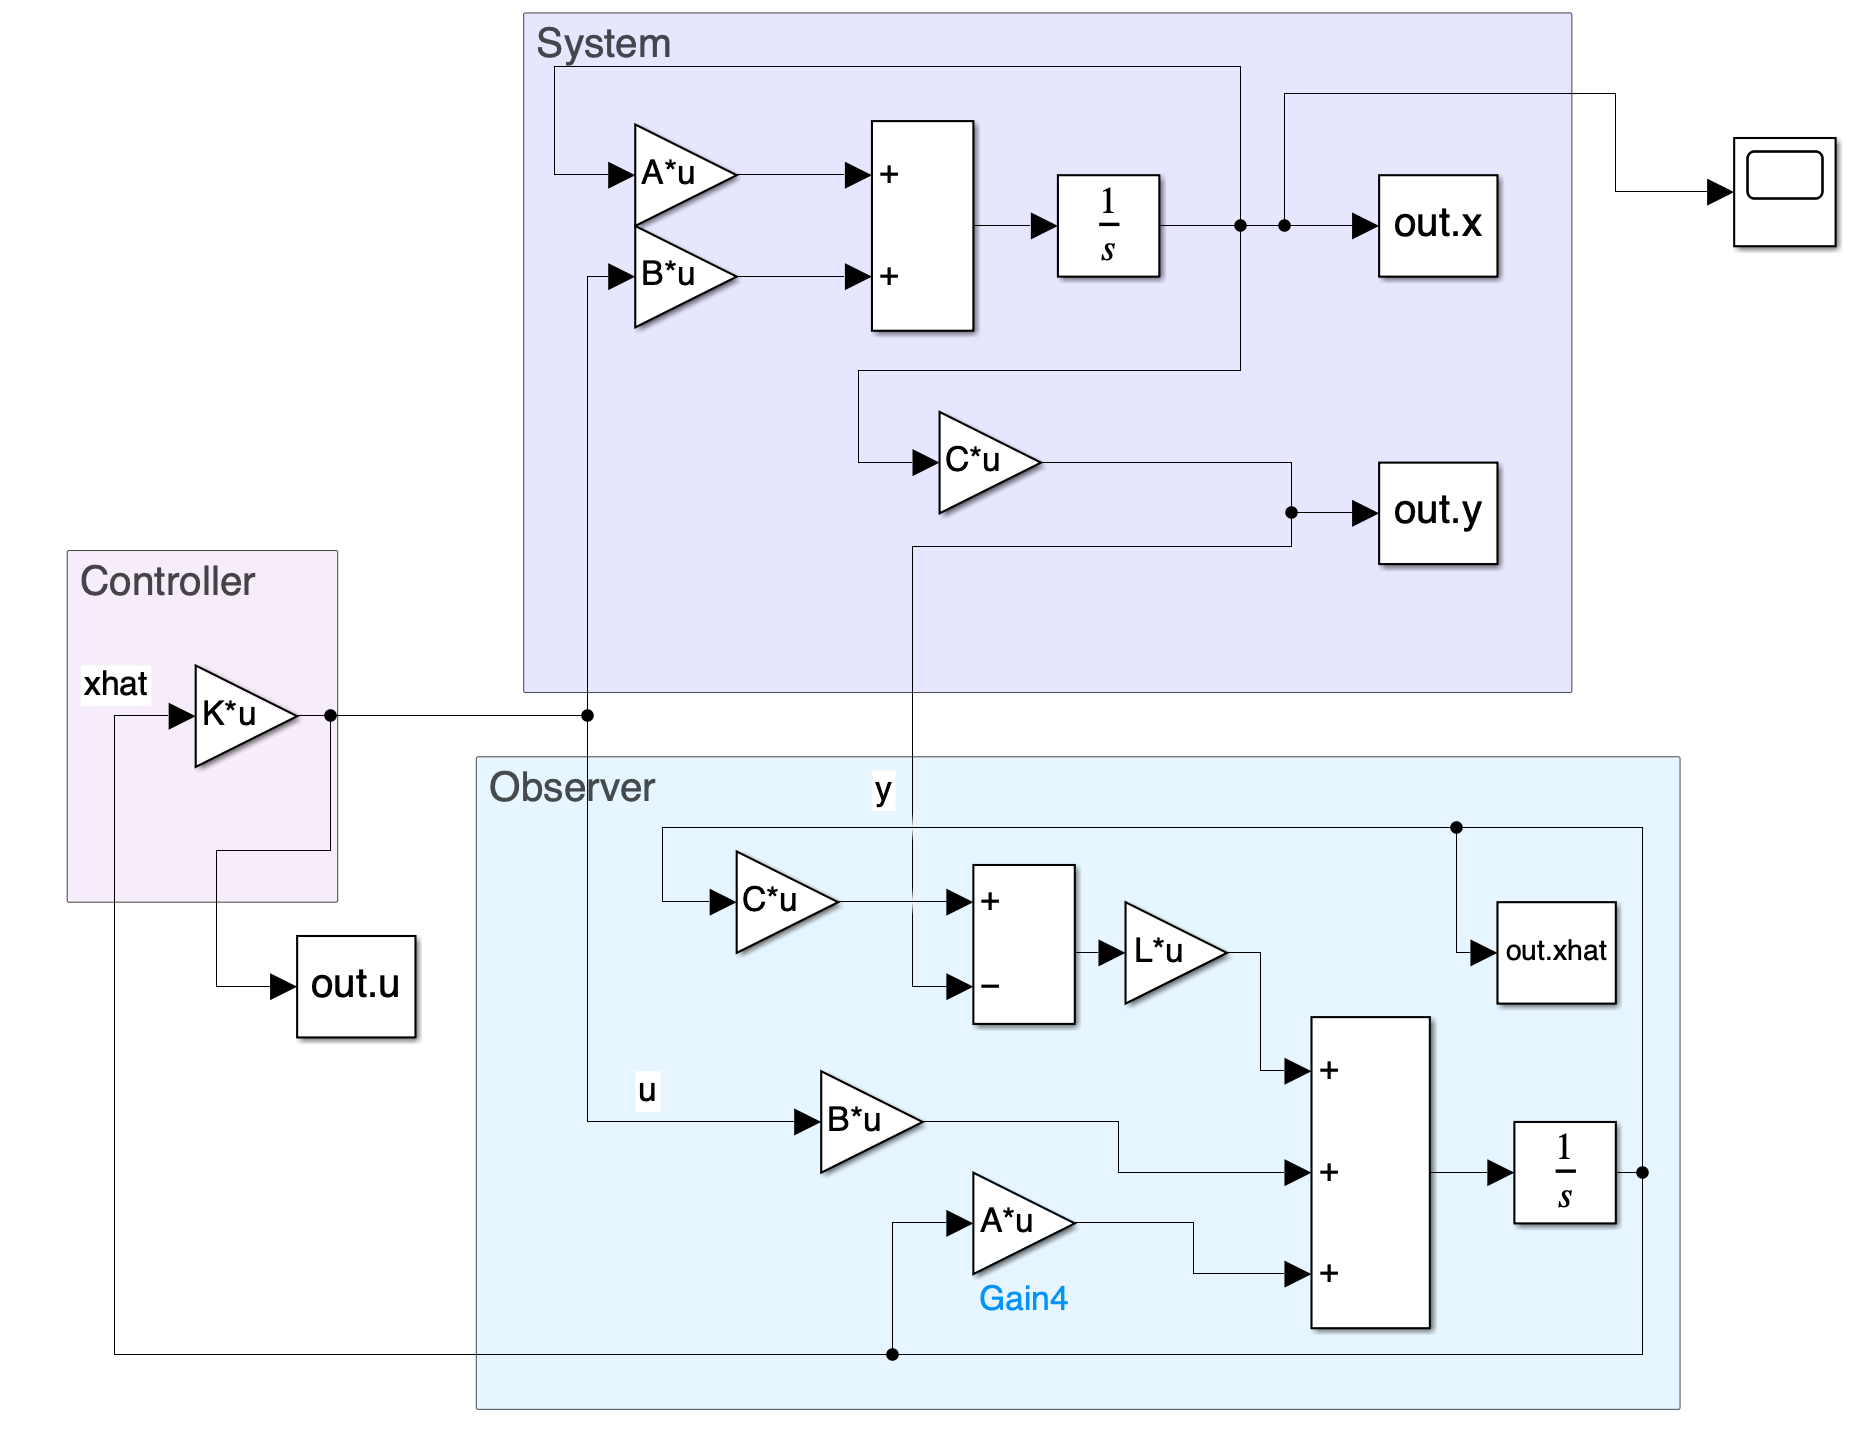
\includegraphics[width=\textwidth]{media/scheme2.png}
    \caption{Схема моделирования системы}
    \label{fig:task2_1_scheme}
\end{figure}

Рассмотрим несколько вариантов систем с разными комбинациями регуляторов и наблюдателей, среди которых 
\begin{itemize}
    \item $K_1$ и $L_1$ -- $12, 12$
    \item $K_1$ и $L_2$ -- $12, 1$
    \item $K_2$ и $L_1$ -- $1, 12$
    \item $K_2$ и $L_2$ -- $1, 1$
\end{itemize}
значения после тире соответствуют степени устойчивости регулятора и наблюдателя.

Таким образом, будут рассмотрены четыре системы, которые будут отличаться только матрицами регулятора и наблюдателя.
При этом среди них будет две системы, в которых степень устойчивости регулятора и наблюдателя равны, 
а также две системы, в которых степень устойчивости регулятора и наблюдателя различны, в одной из которых
степень устойчивости регулятора больше степени устойчивости наблюдателя, а в другой наоборот.

Проведем моделирование описанных систем. В качестве начальных условий для системы выберем $x_0 = [1, 1, 1, 1]^T$, 
для наблюдателя $\hat{x}_0 = [0, 0, 0, 0]^T$. 
\FloatBarrier
Для регулятора $K_1$ и наблюдателя $L_1$ результаты моделирования представлены на рисунках \ref{fig:task2_1_1_x} 
(состояние системы), \ref{fig:task2_1_1_e} (ошибка наблюдения), \ref{fig:task2_1_1_u} (управляющее воздействие) и \ref{fig:task2_1_1_xh} 
(состояние системы и ее оценка).
\begin{figure}[ht!]
    \centering
    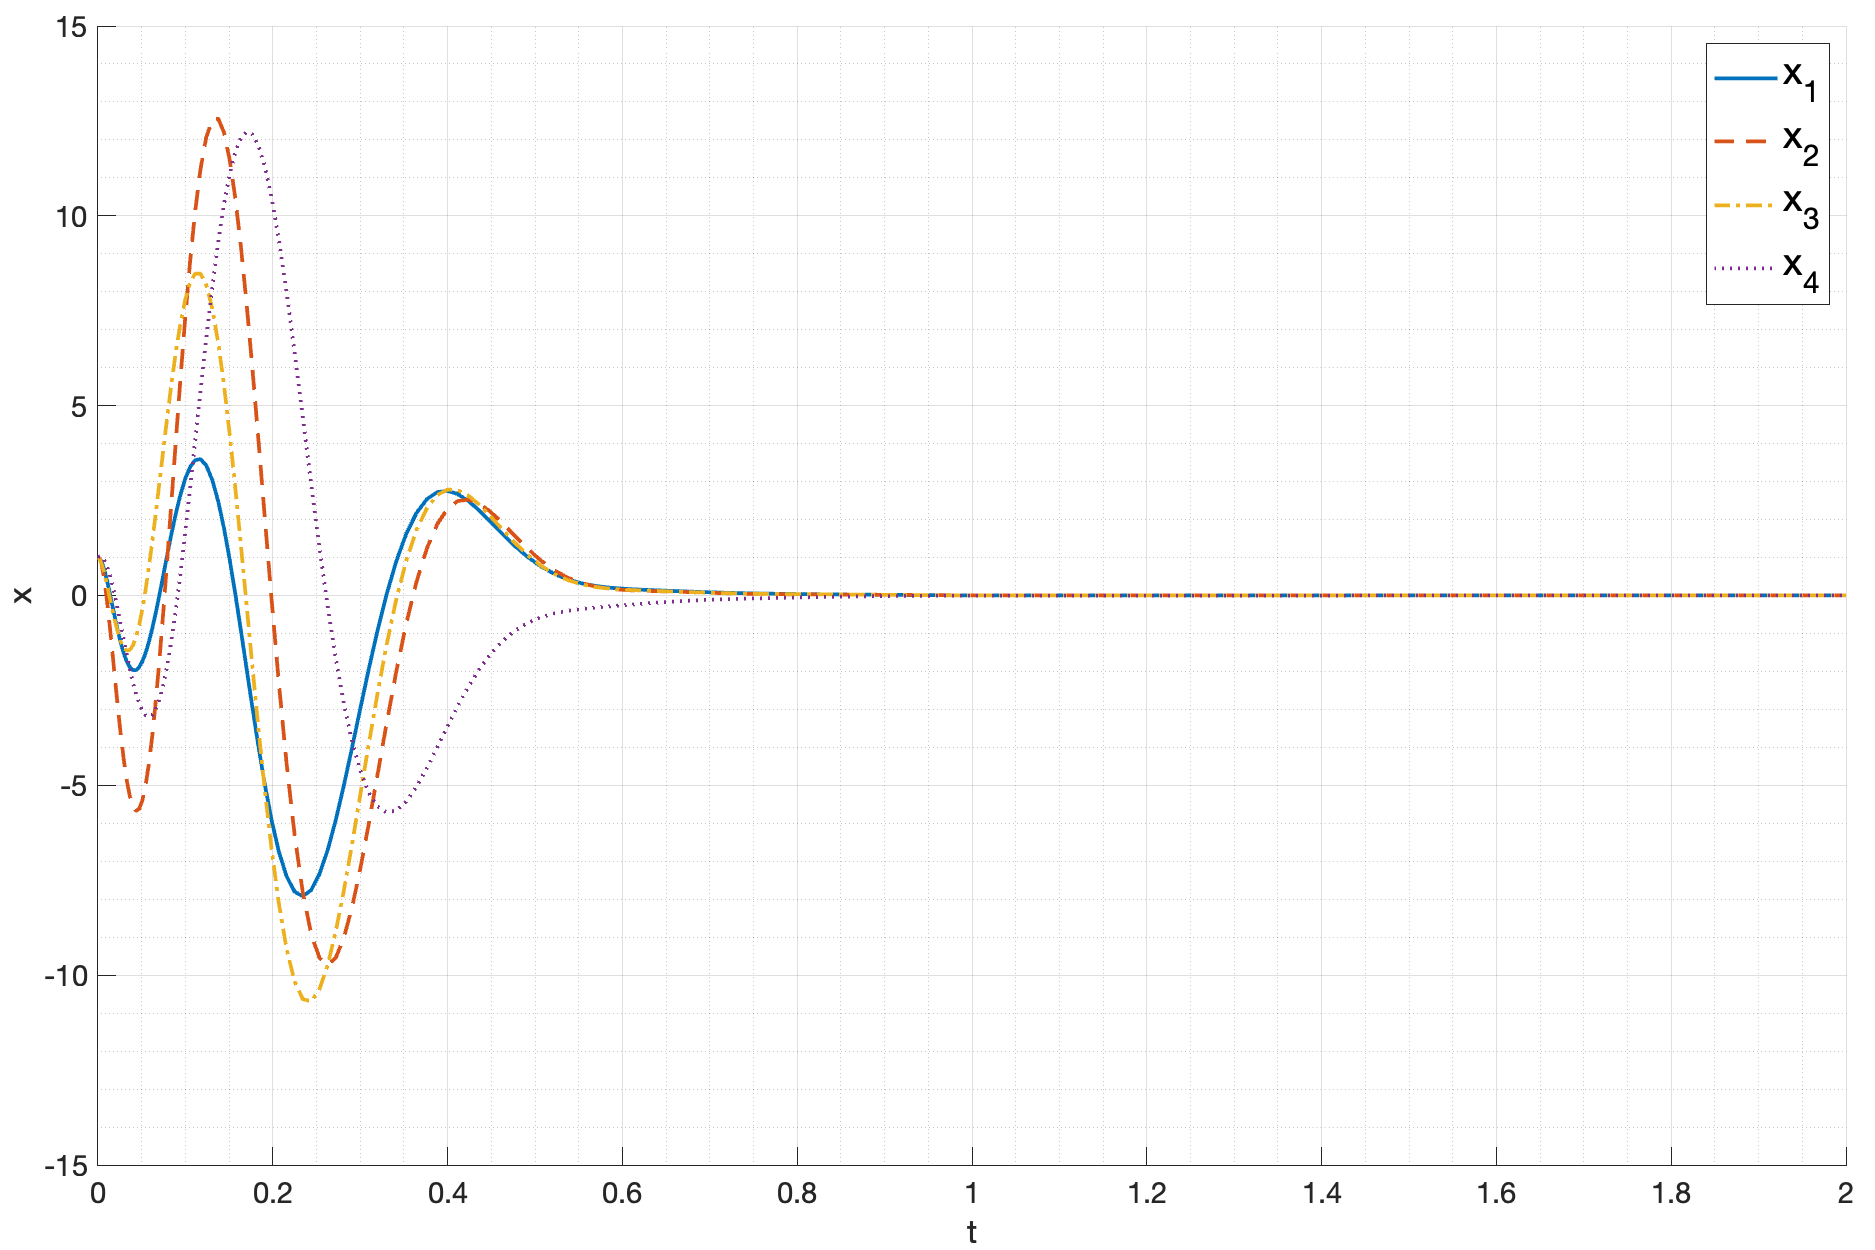
\includegraphics[width=\textwidth]{media/plots/task2_1_x.png}
    \caption{Состояние системы $K_1$ и $L_1$}
    \label{fig:task2_1_1_x}
\end{figure}
\begin{figure}[ht!]
    \centering
    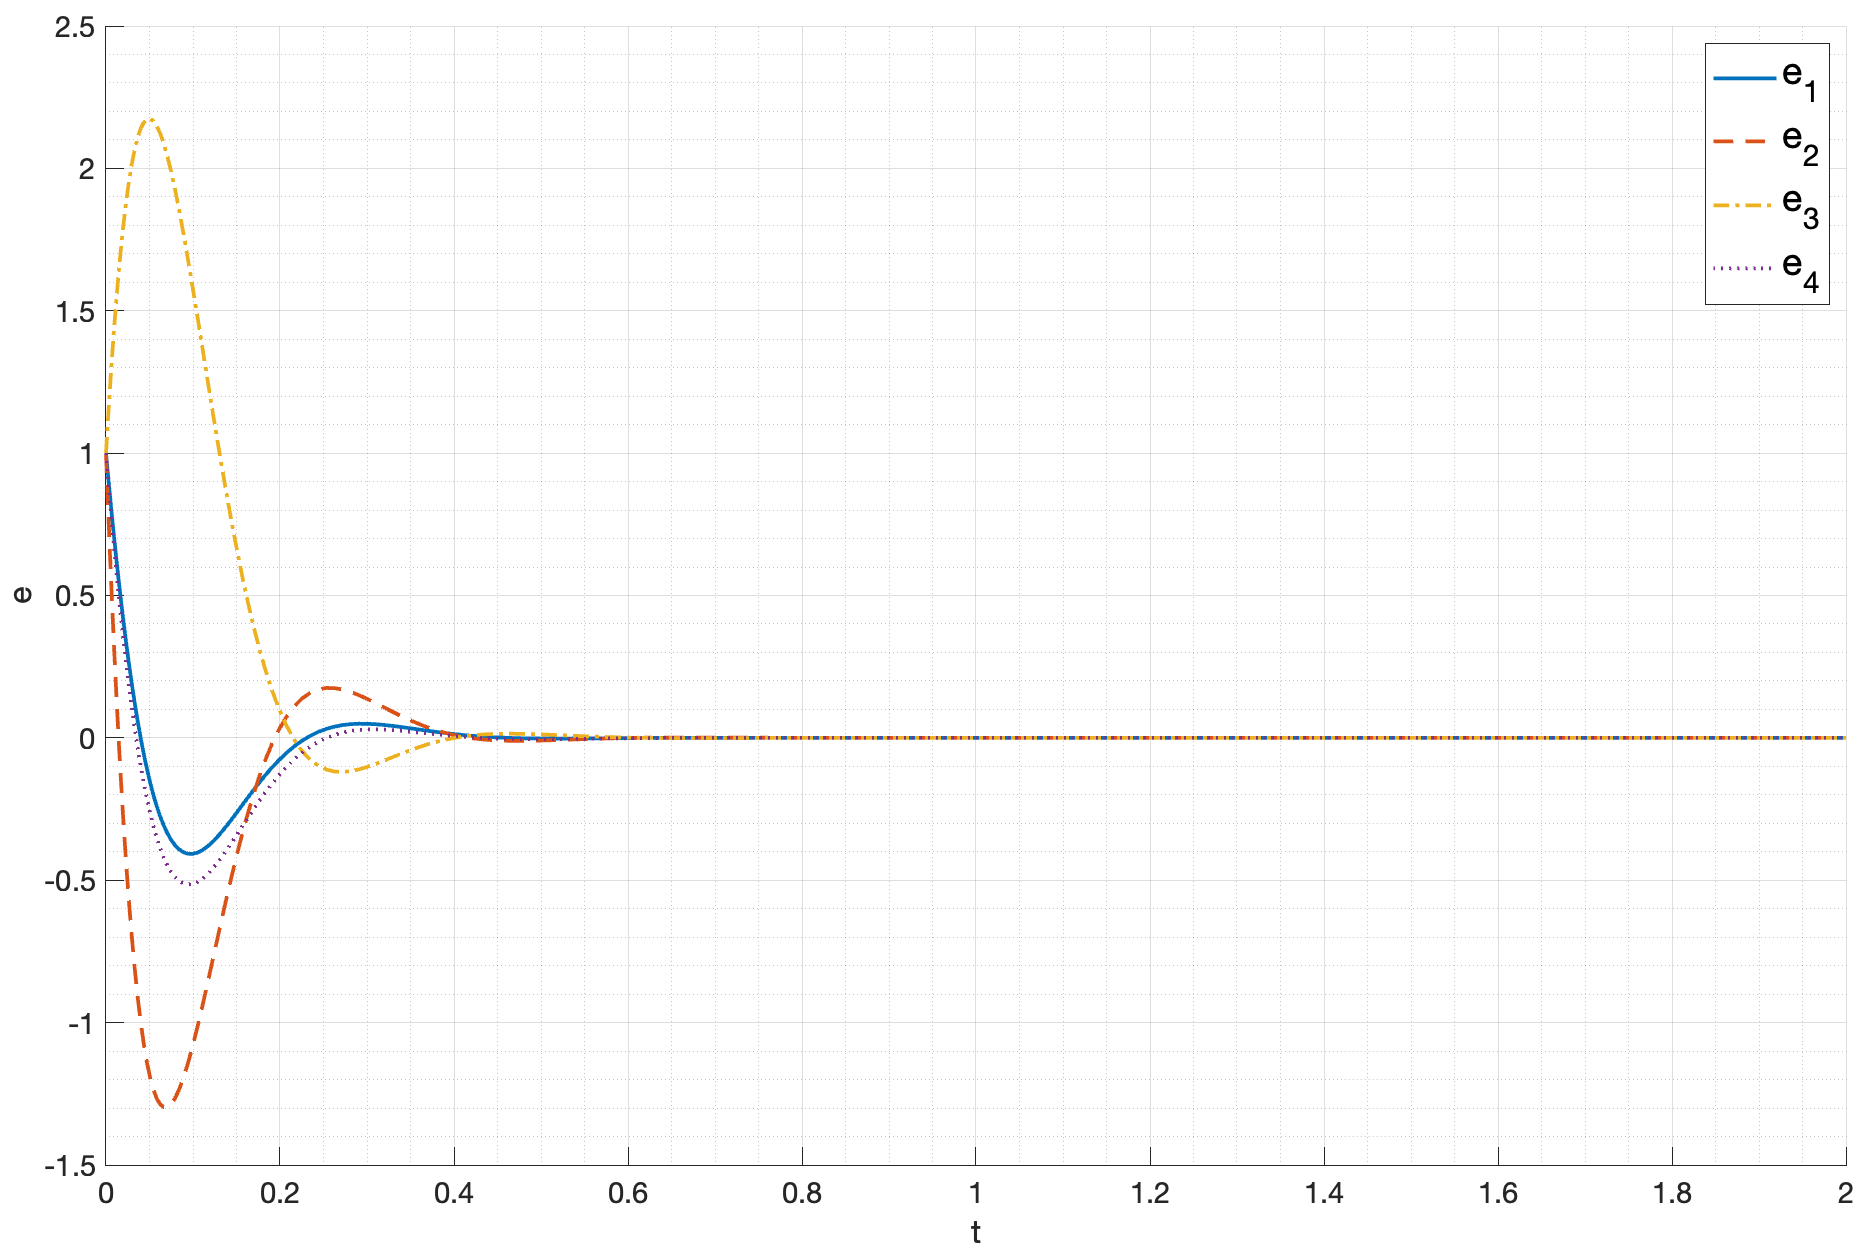
\includegraphics[width=\textwidth]{media/plots/task2_1_e.png}
    \caption{Ошибка наблюдения $K_1$ и $L_1$}
    \label{fig:task2_1_1_e}
\end{figure}
\begin{figure}[ht!]
    \centering
    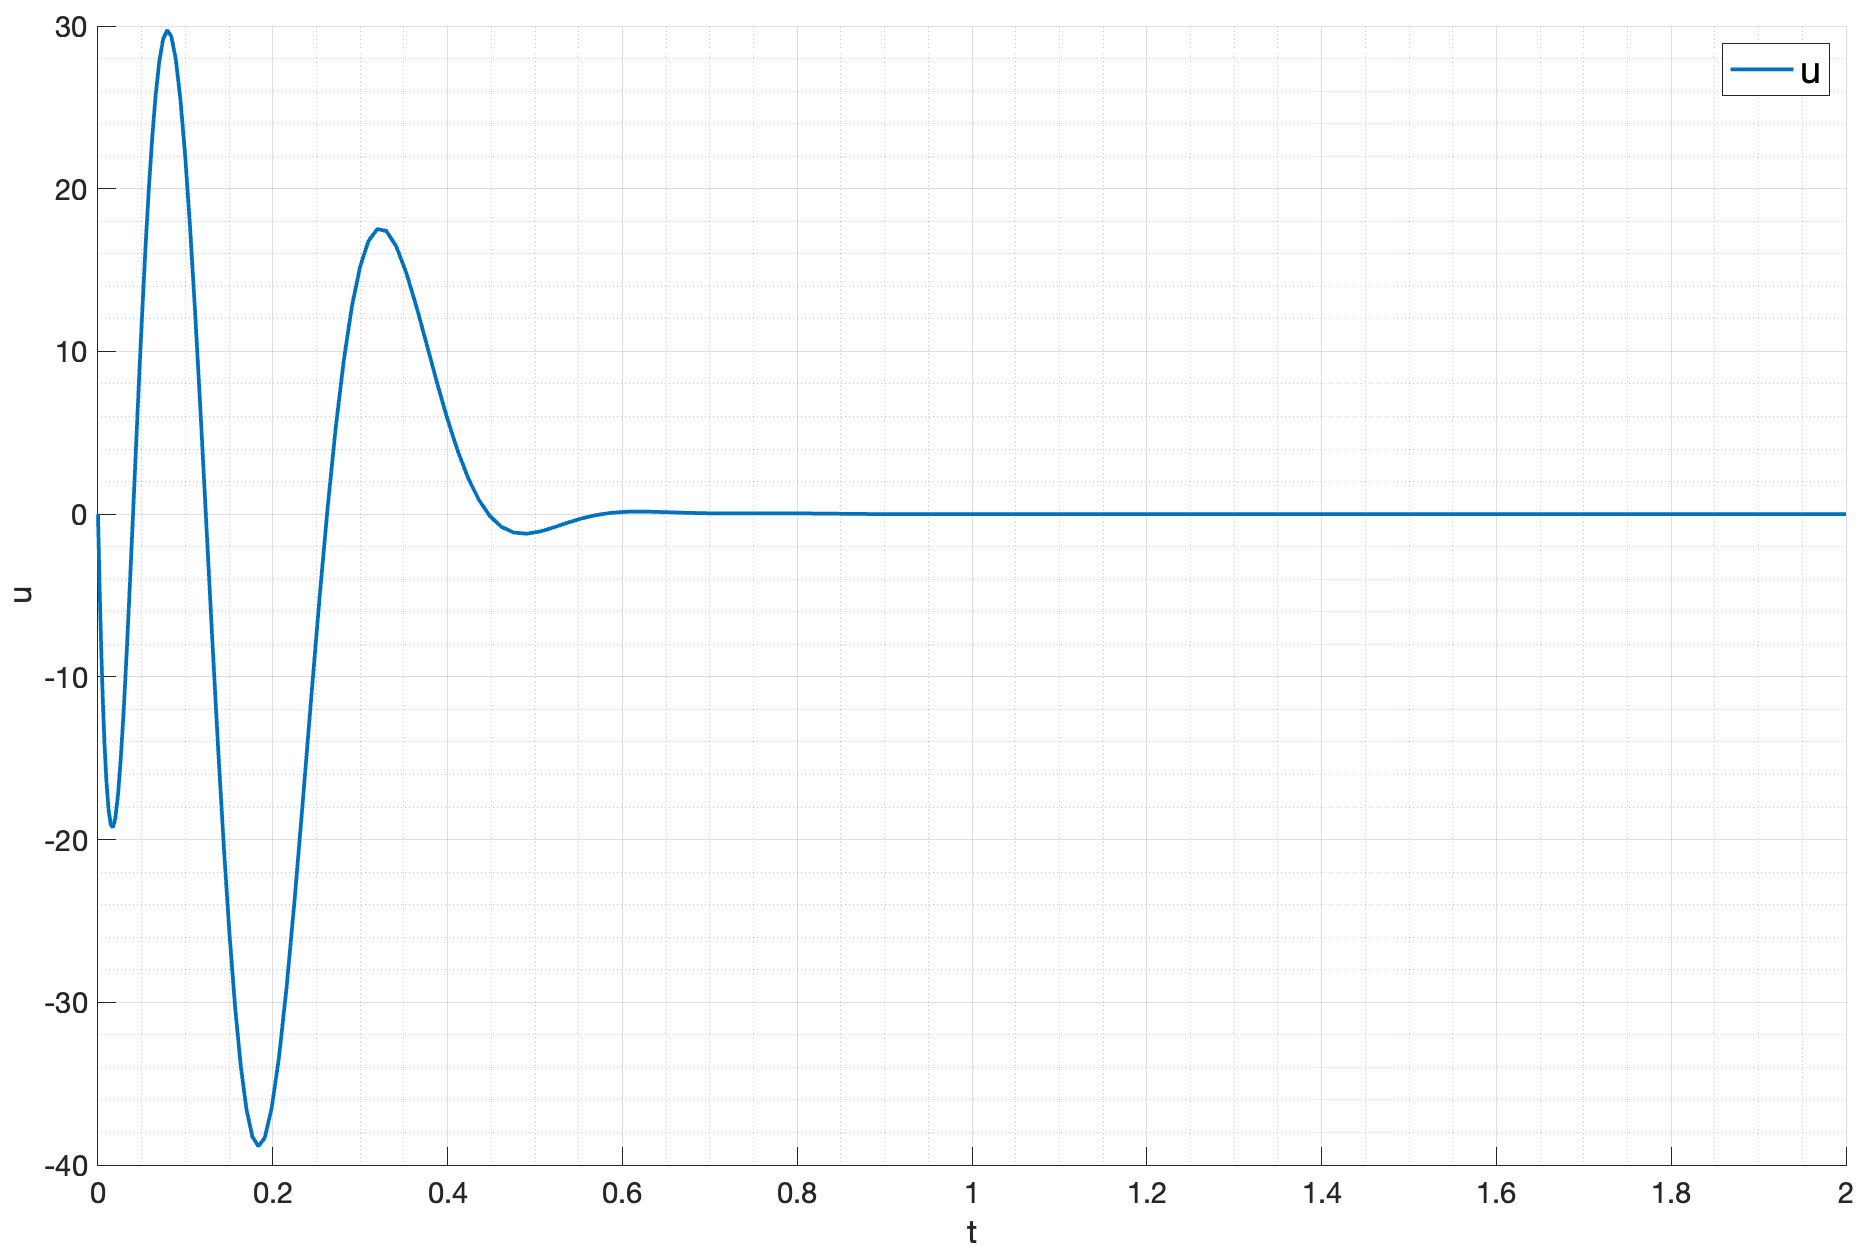
\includegraphics[width=\textwidth]{media/plots/task2_1_u.png}
    \caption{Управляющее воздействие $K_1$ и $L_1$}
    \label{fig:task2_1_1_u}
\end{figure}
\begin{figure}[ht!]
    \centering
    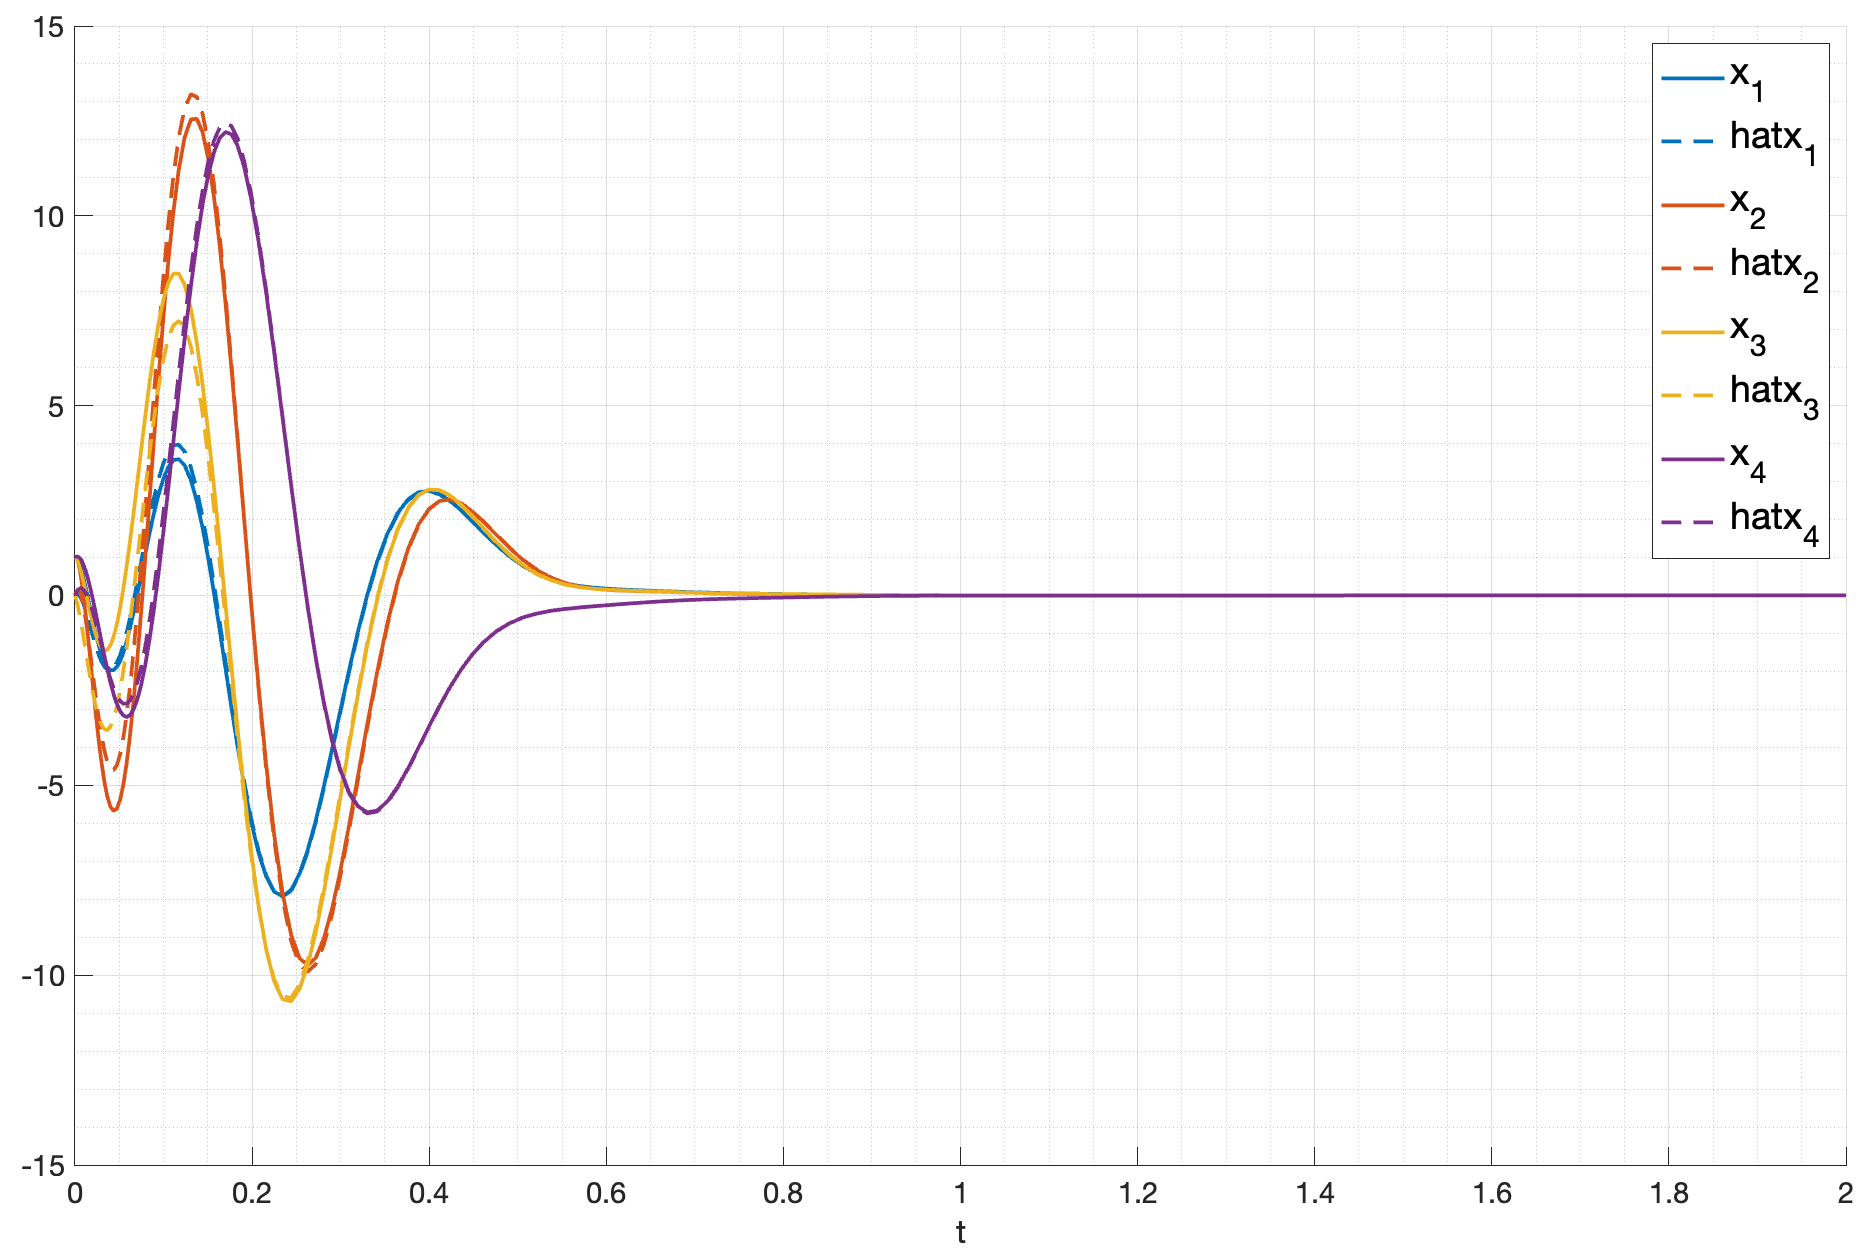
\includegraphics[width=\textwidth]{media/plots/task2_1_xh.png}
    \caption{Состояние системы и ее оценка $K_1$ и $L_1$}
    \label{fig:task2_1_1_xh}
\end{figure}
\FloatBarrier

Для регулятора $K_1$ и наблюдателя $L_2$ результаты моделирования представлены на рисунках \ref{fig:task2_1_2_x} 
(состояние системы), \ref{fig:task2_1_2_e} (ошибка наблюдения), \ref{fig:task2_1_2_u} (управляющее воздействие) и \ref{fig:task2_1_2_xh} 
(состояние системы и ее оценка).
\begin{figure}[ht!]
    \centering
    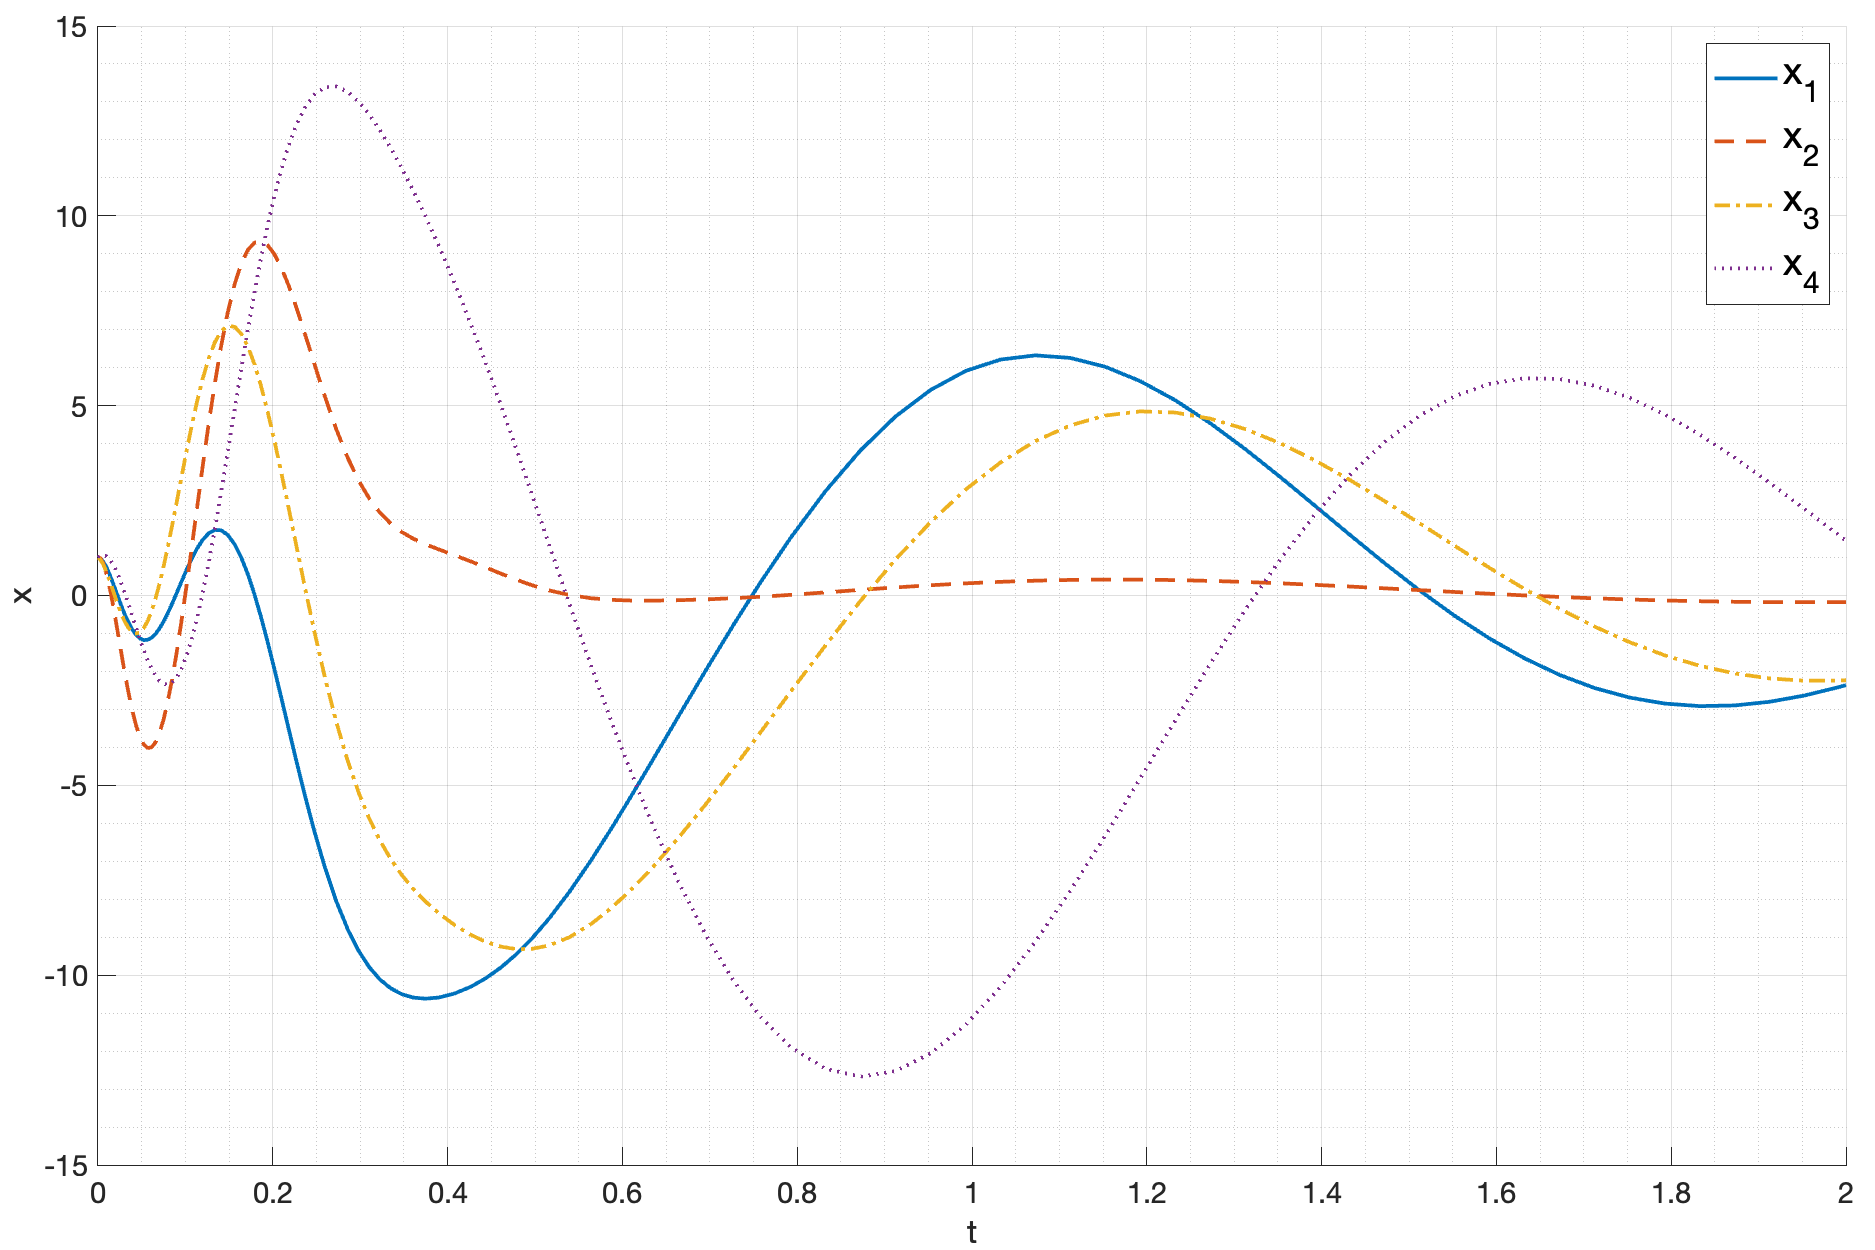
\includegraphics[width=\textwidth]{media/plots/task2_2_x.png}
    \caption{Состояние системы $K_1$ и $L_2$}
    \label{fig:task2_1_2_x}
\end{figure}
\begin{figure}[ht!]
    \centering
    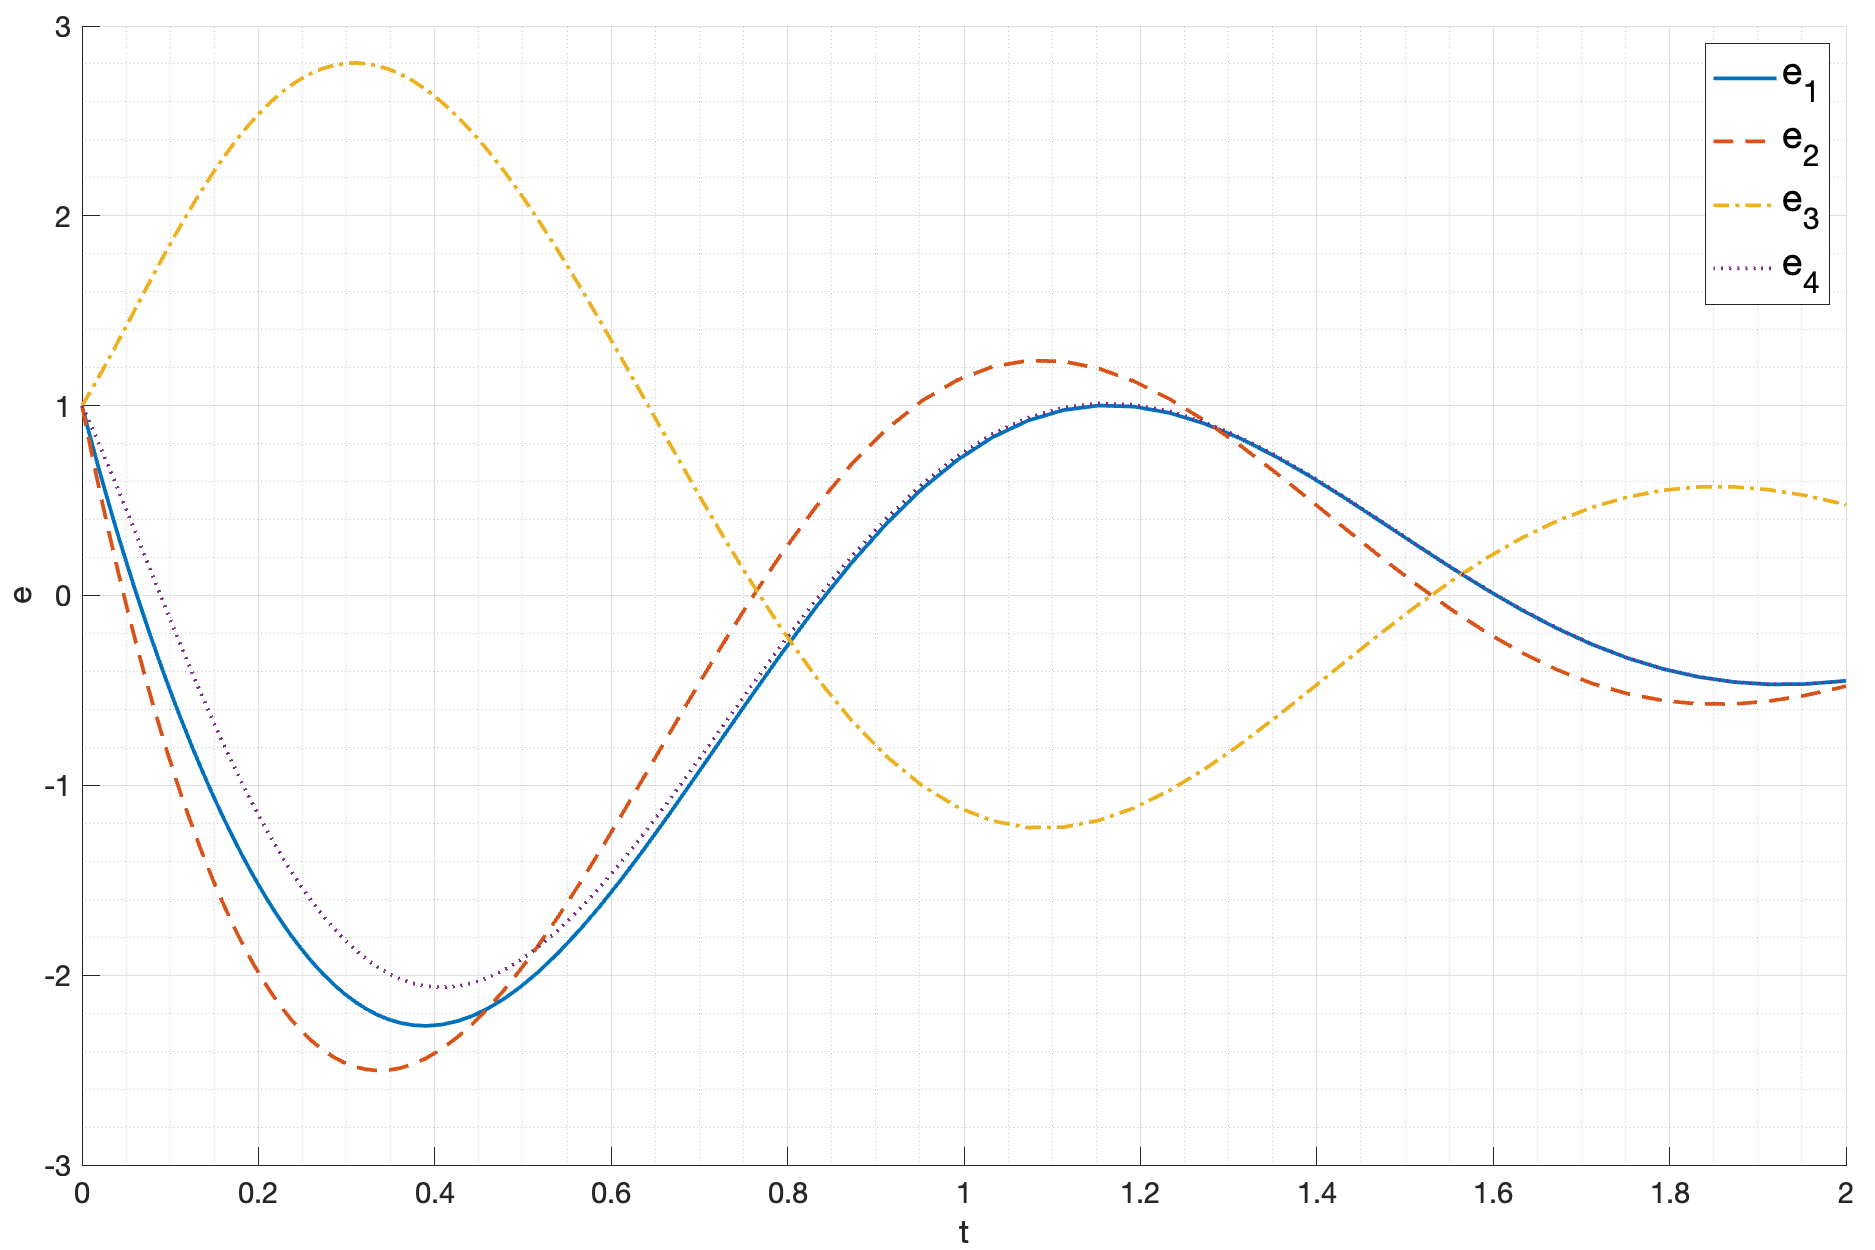
\includegraphics[width=\textwidth]{media/plots/task2_2_e.png}
    \caption{Ошибка наблюдения $K_1$ и $L_2$}
    \label{fig:task2_1_2_e}
\end{figure}
\begin{figure}[ht!]
    \centering
    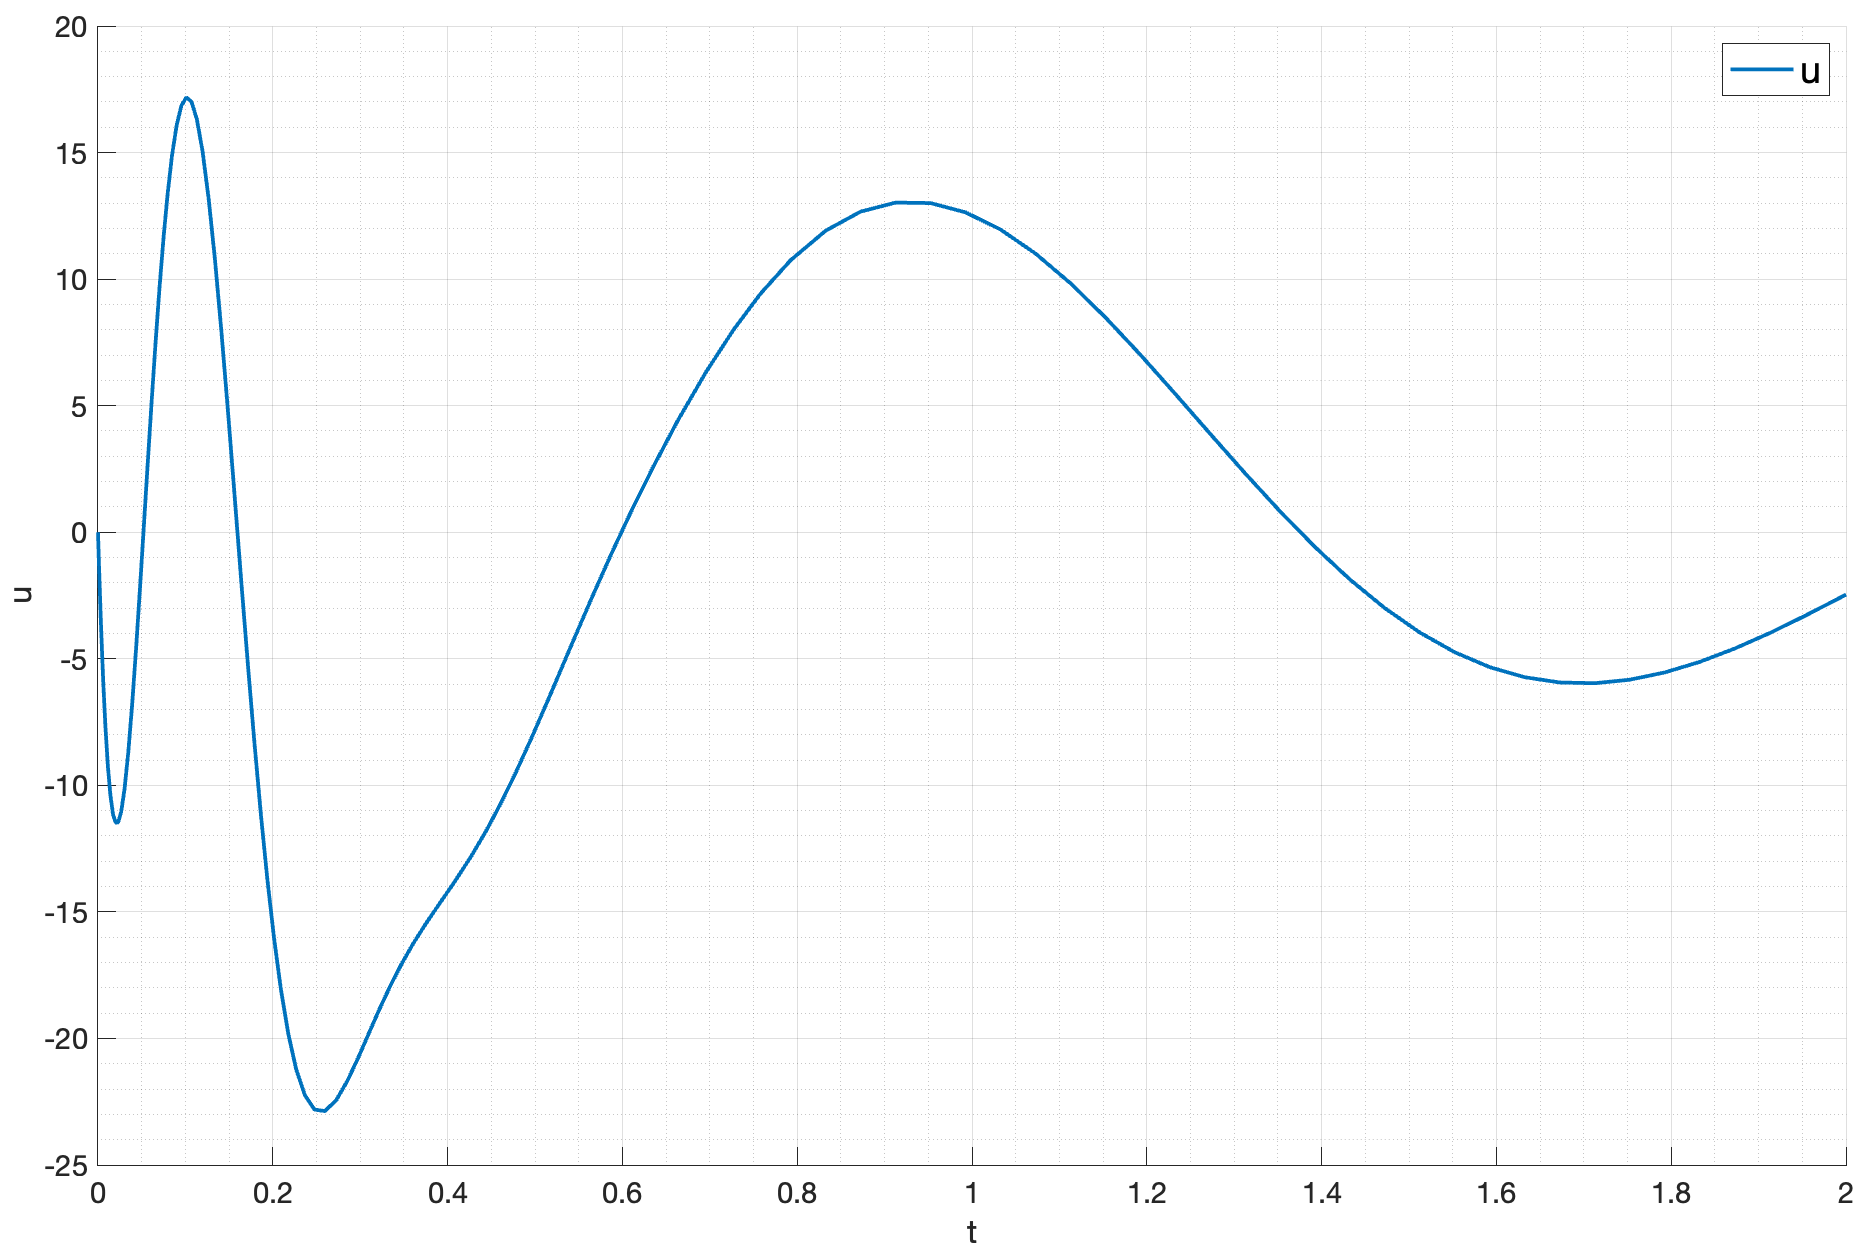
\includegraphics[width=\textwidth]{media/plots/task2_2_u.png}
    \caption{Управляющее воздействие $K_1$ и $L_2$}
    \label{fig:task2_1_2_u}
\end{figure}
\begin{figure}[ht!]
    \centering
    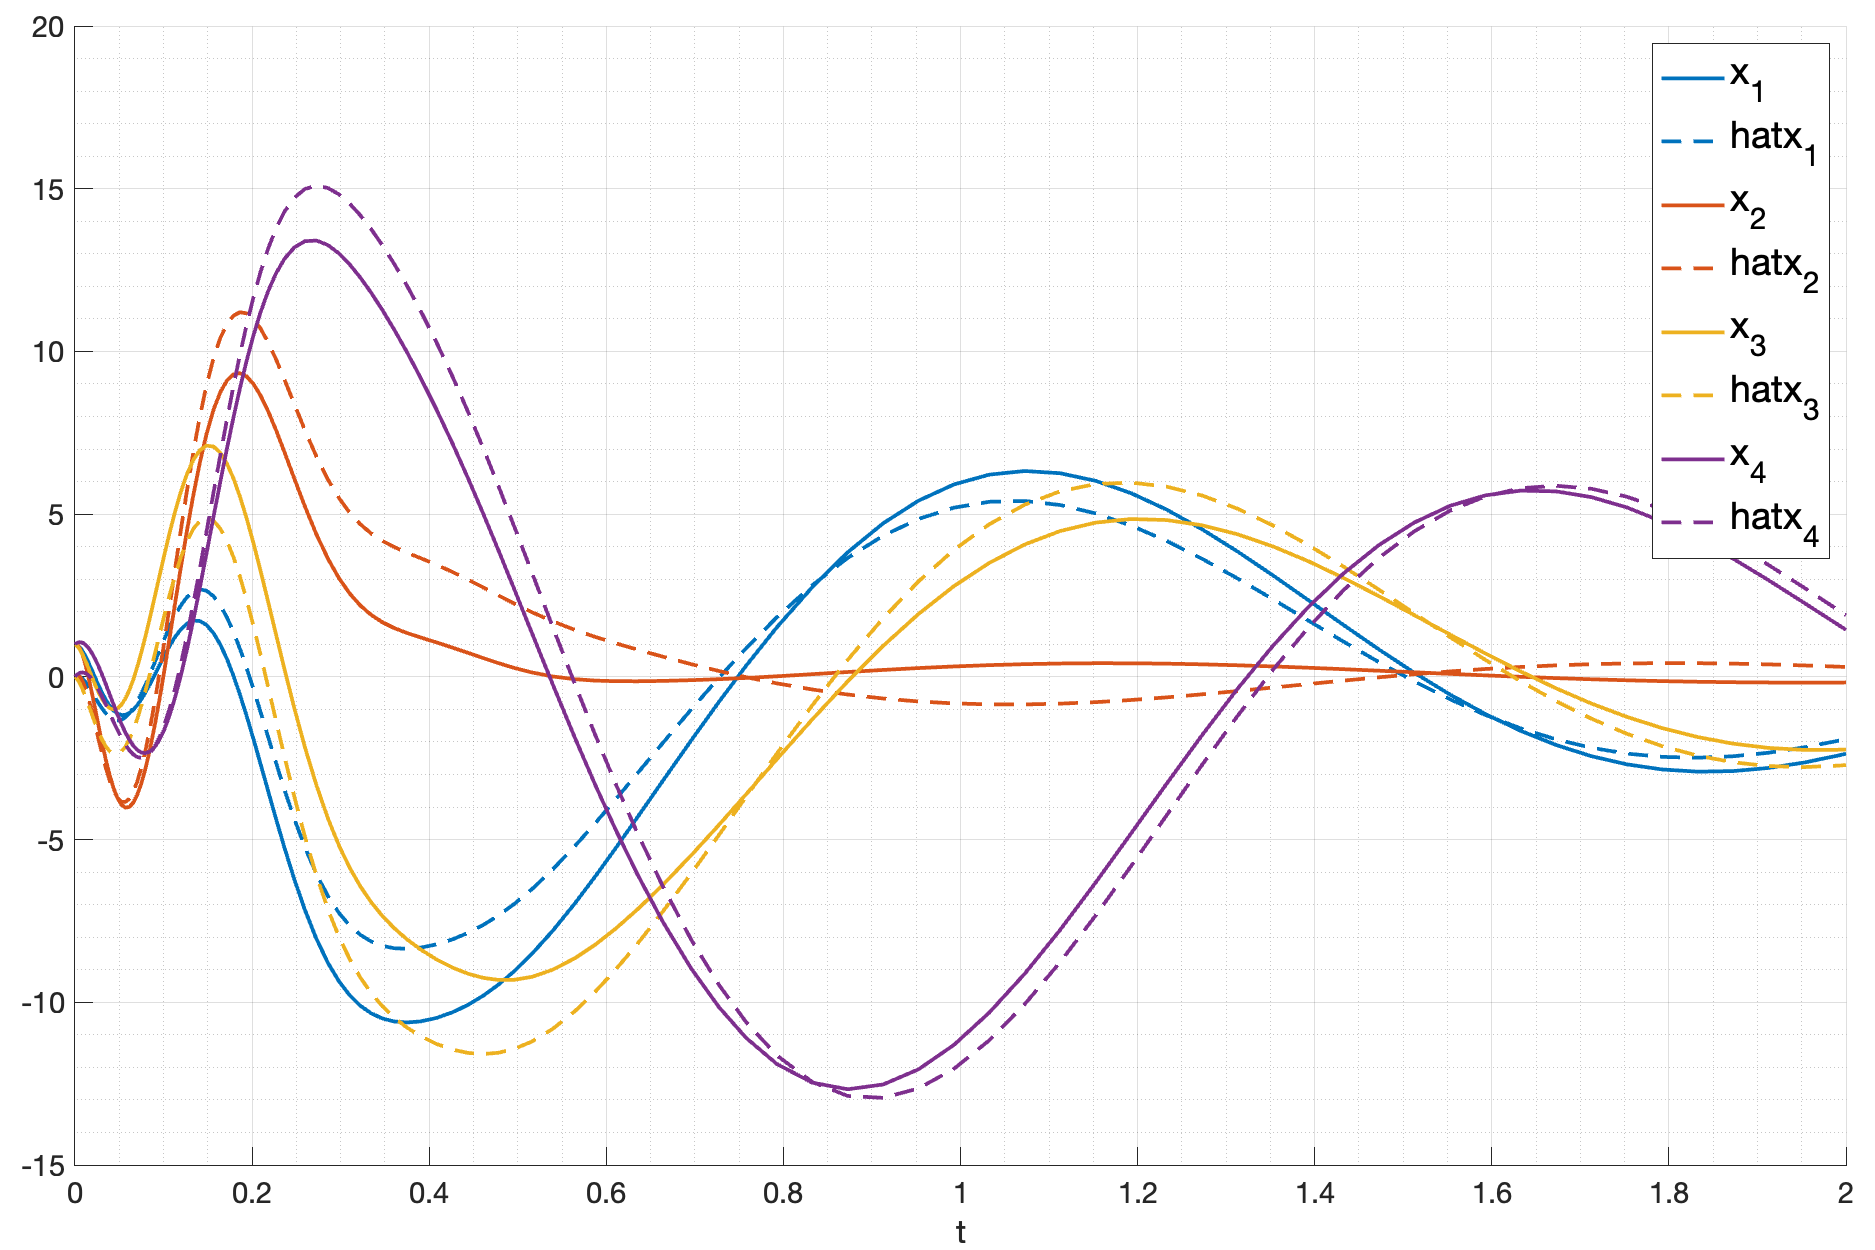
\includegraphics[width=\textwidth]{media/plots/task2_2_xh.png}
    \caption{Состояние системы и ее оценка $K_1$ и $L_2$}
    \label{fig:task2_1_2_xh}
\end{figure}
\FloatBarrier

Для регулятора $K_2$ и наблюдателя $L_1$ результаты моделирования представлены на рисунках \ref{fig:task2_2_1_x} 
(состояние системы), \ref{fig:task2_2_1_e} (ошибка наблюдения), \ref{fig:task2_2_1_u} (управляющее воздействие) и \ref{fig:task2_2_1_xh} 
(состояние системы и ее оценка).

\begin{figure}[ht!]
    \centering
    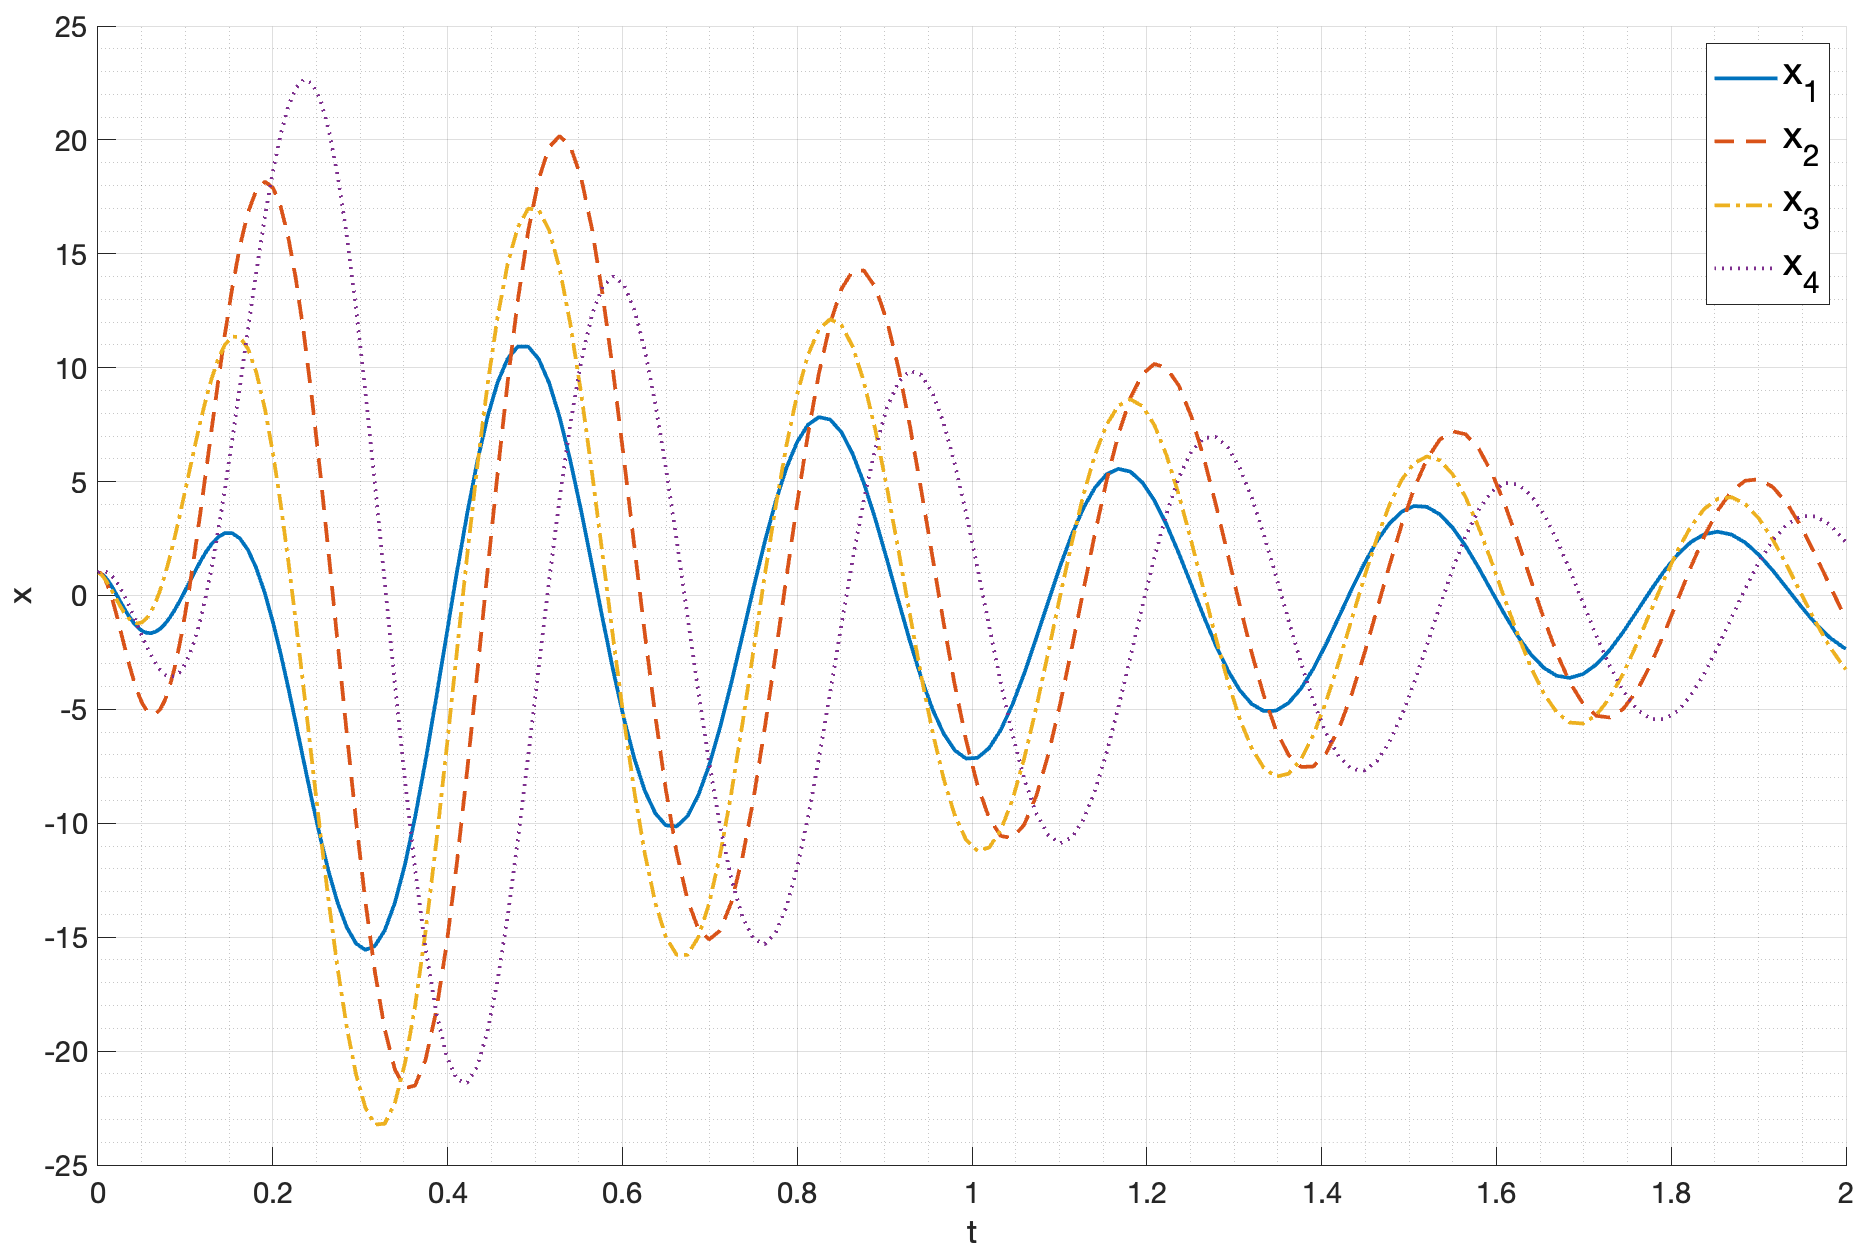
\includegraphics[width=\textwidth]{media/plots/task2_3_x.png}
    \caption{Состояние системы $K_2$ и $L_1$}
    \label{fig:task2_2_1_x}
\end{figure}
\begin{figure}[ht!]
    \centering
    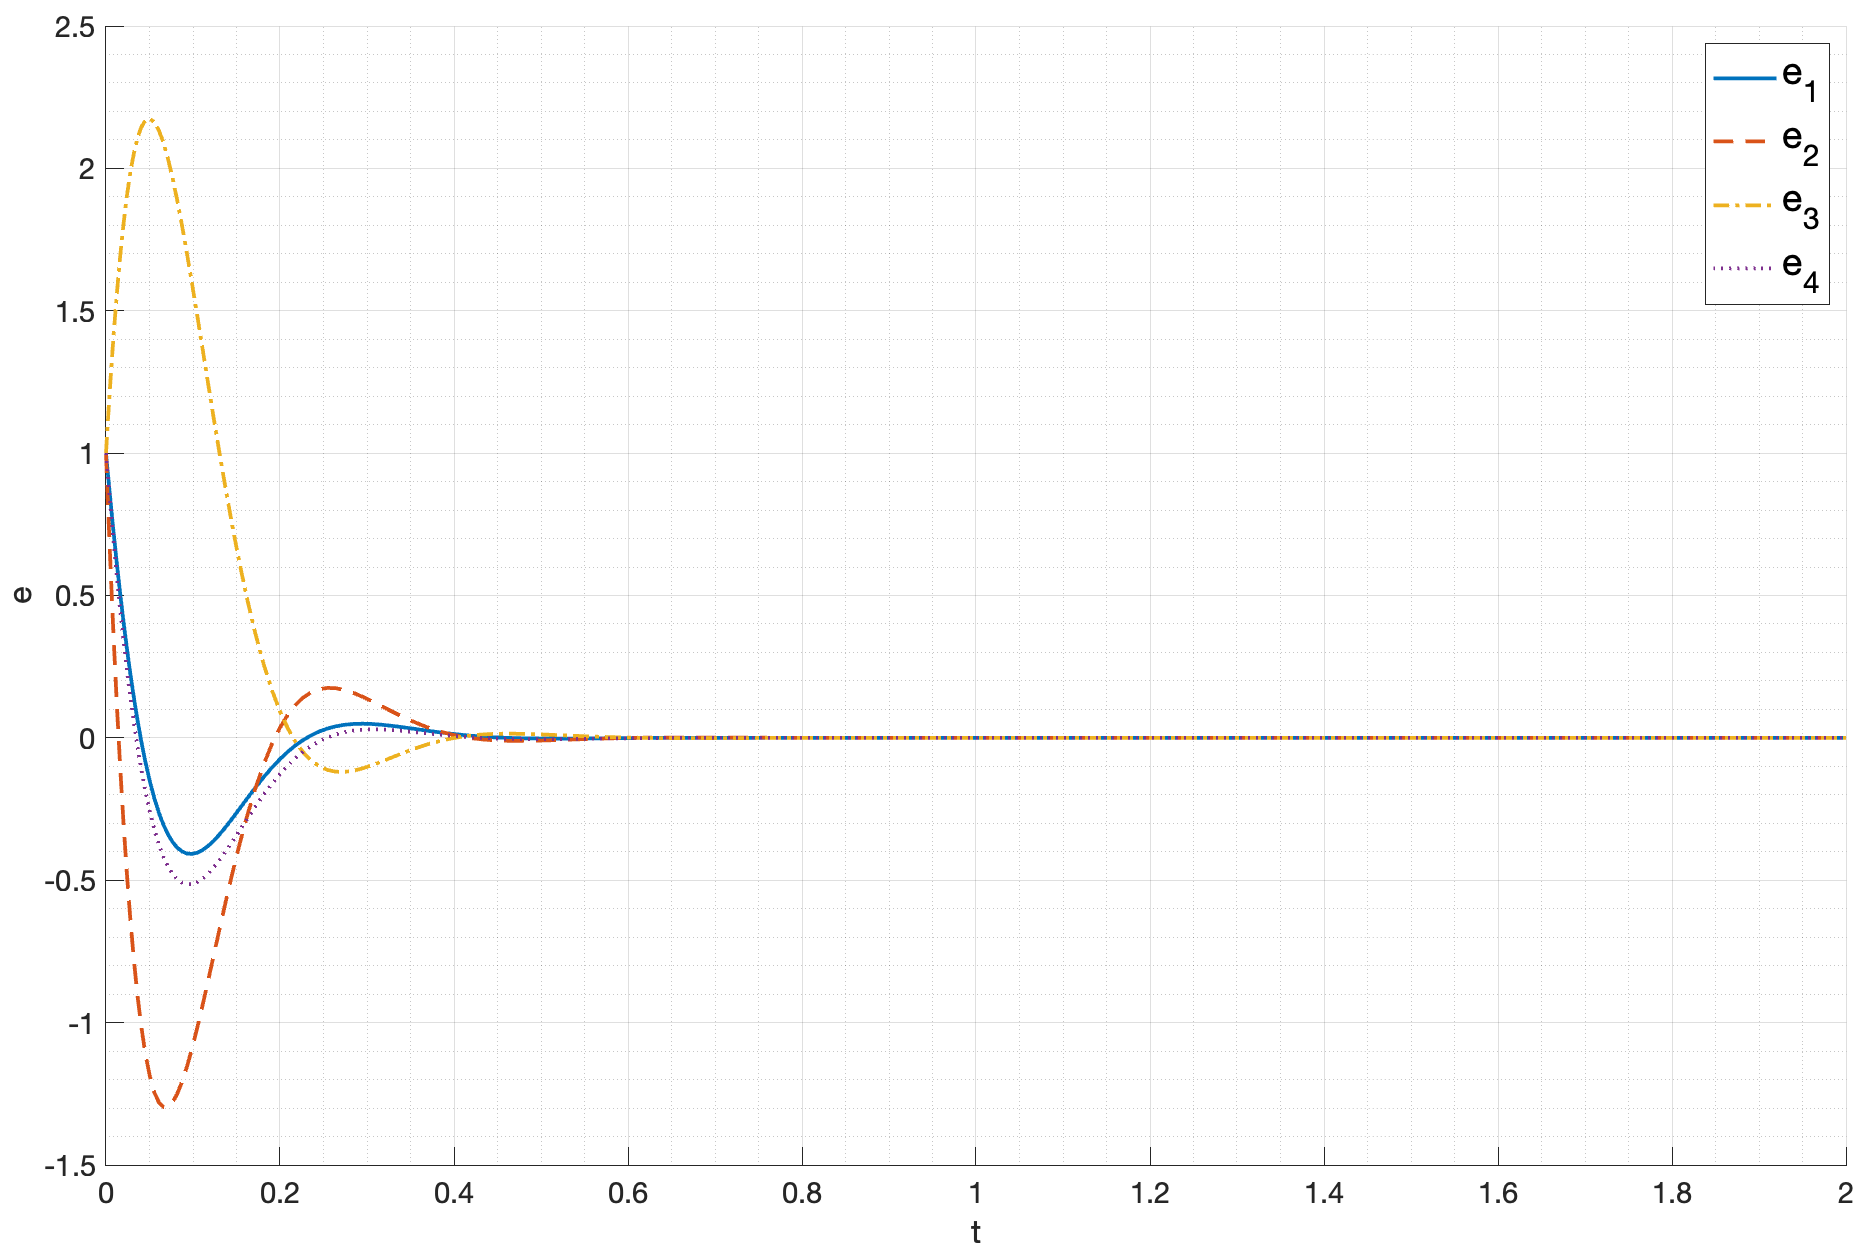
\includegraphics[width=\textwidth]{media/plots/task2_3_e.png}
    \caption{Ошибка наблюдения $K_2$ и $L_1$}
    \label{fig:task2_2_1_e}
\end{figure}
\begin{figure}[ht!]
    \centering
    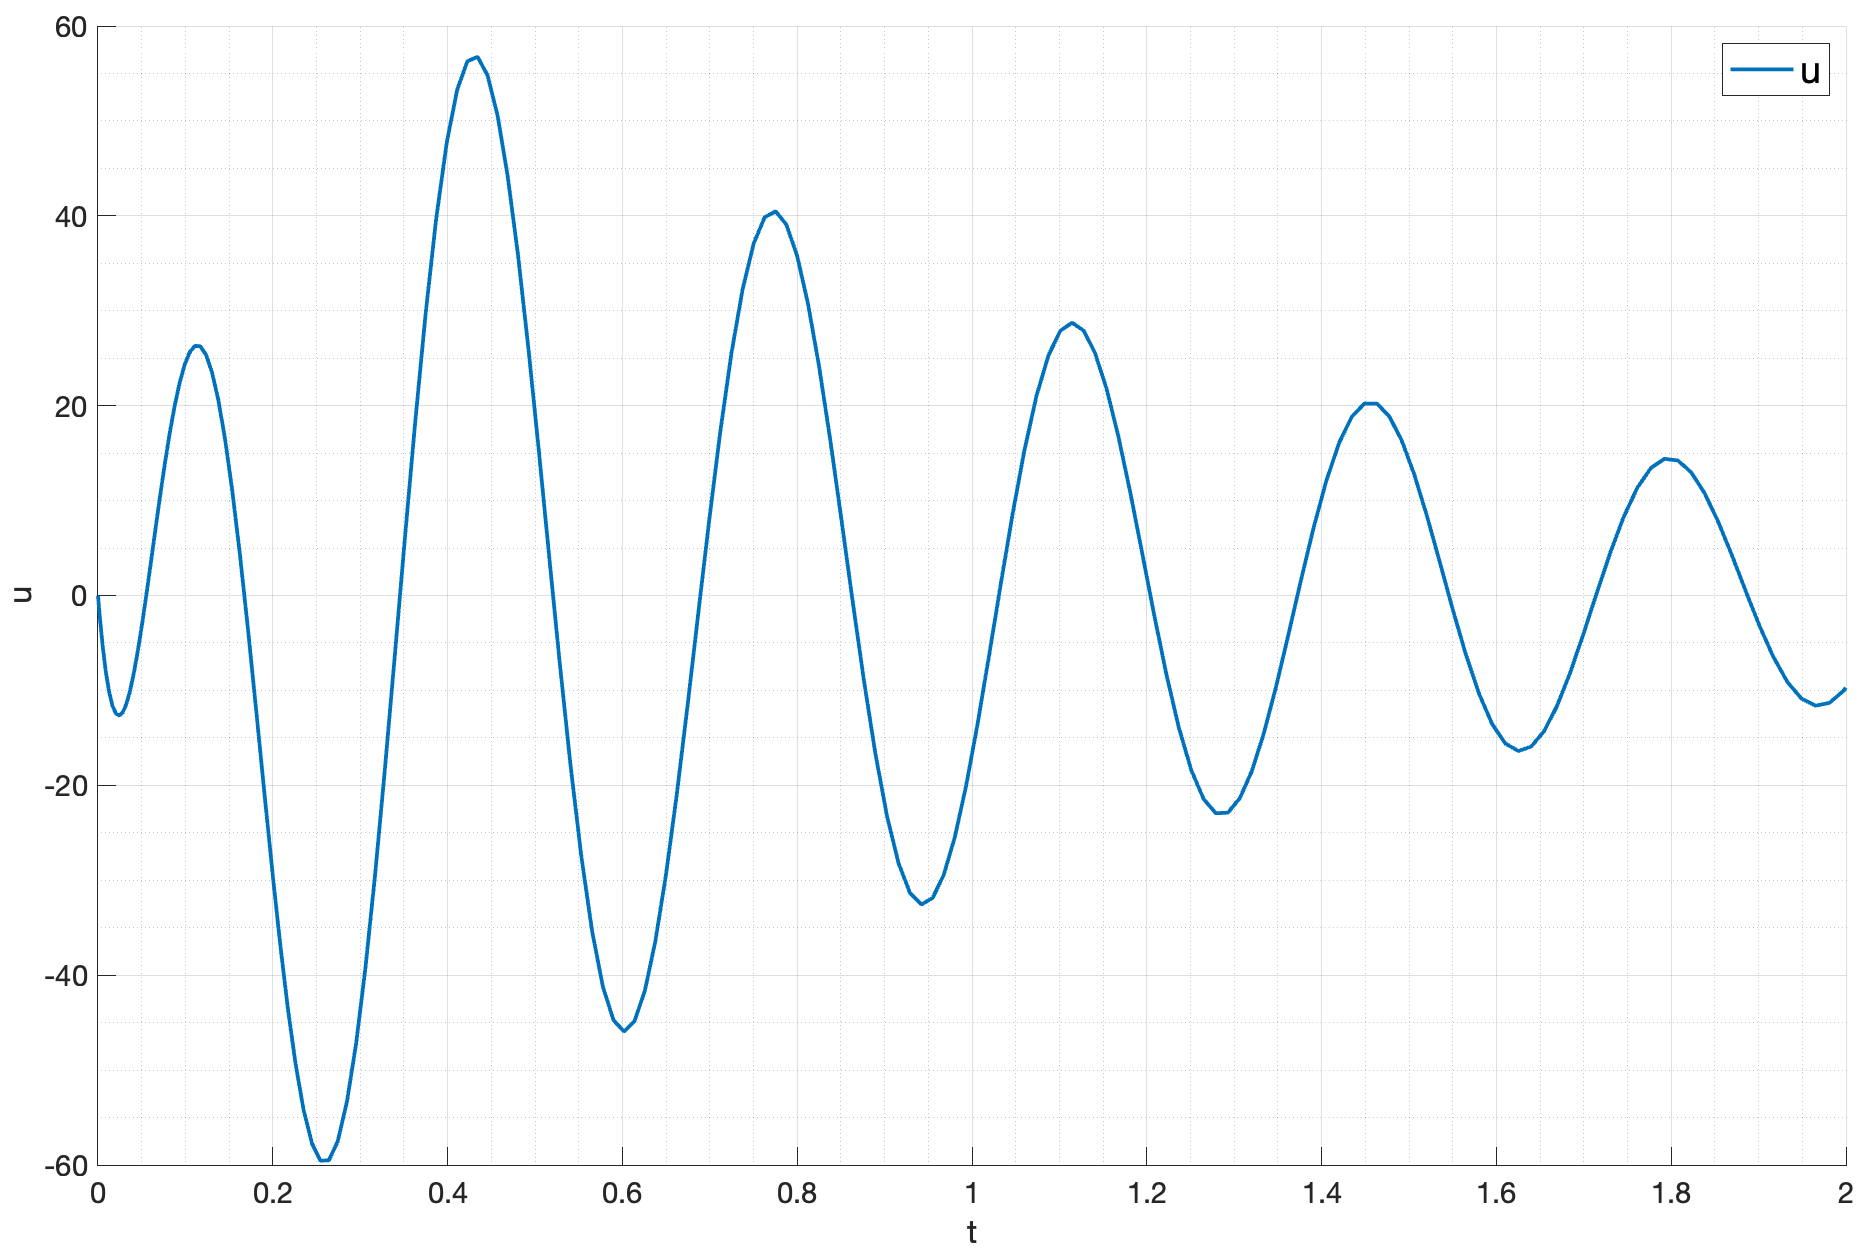
\includegraphics[width=\textwidth]{media/plots/task2_3_u.png}
    \caption{Управляющее воздействие $K_2$ и $L_1$}
    \label{fig:task2_2_1_u}
\end{figure}
\begin{figure}[ht!]
    \centering
    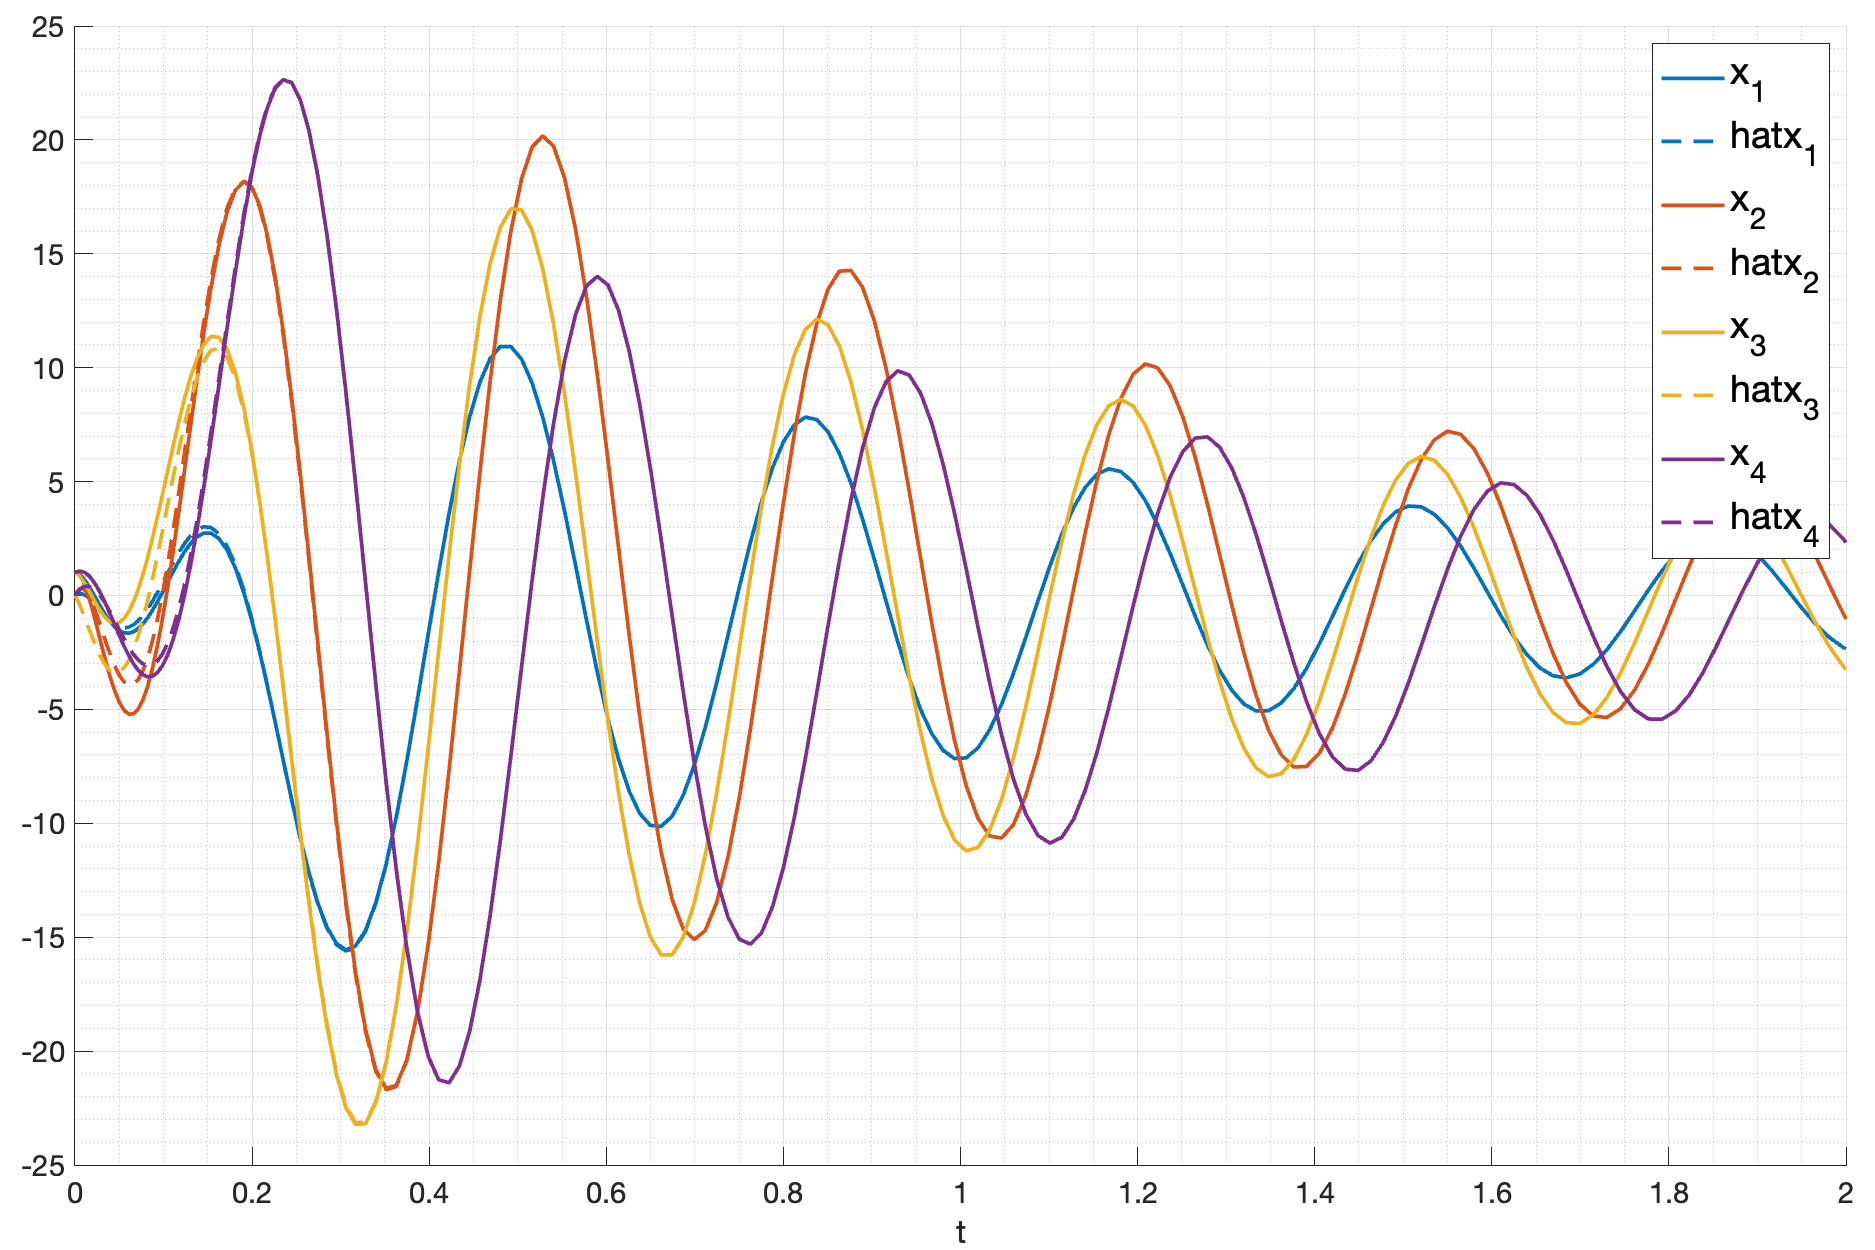
\includegraphics[width=\textwidth]{media/plots/task2_3_xh.png}
    \caption{Состояние системы и ее оценка $K_2$ и $L_1$}
    \label{fig:task2_2_1_xh}
\end{figure}
\FloatBarrier

Для регулятора $K_2$ и наблюдателя $L_2$ результаты моделирования представлены на рисунках \ref{fig:task2_2_2_x} 
(состояние системы), \ref{fig:task2_2_2_e} (ошибка наблюдения), \ref{fig:task2_2_2_u} (управляющее воздействие) и \ref{fig:task2_2_2_xh} 
(состояние системы и ее оценка).
\begin{figure}[ht!]
    \centering
    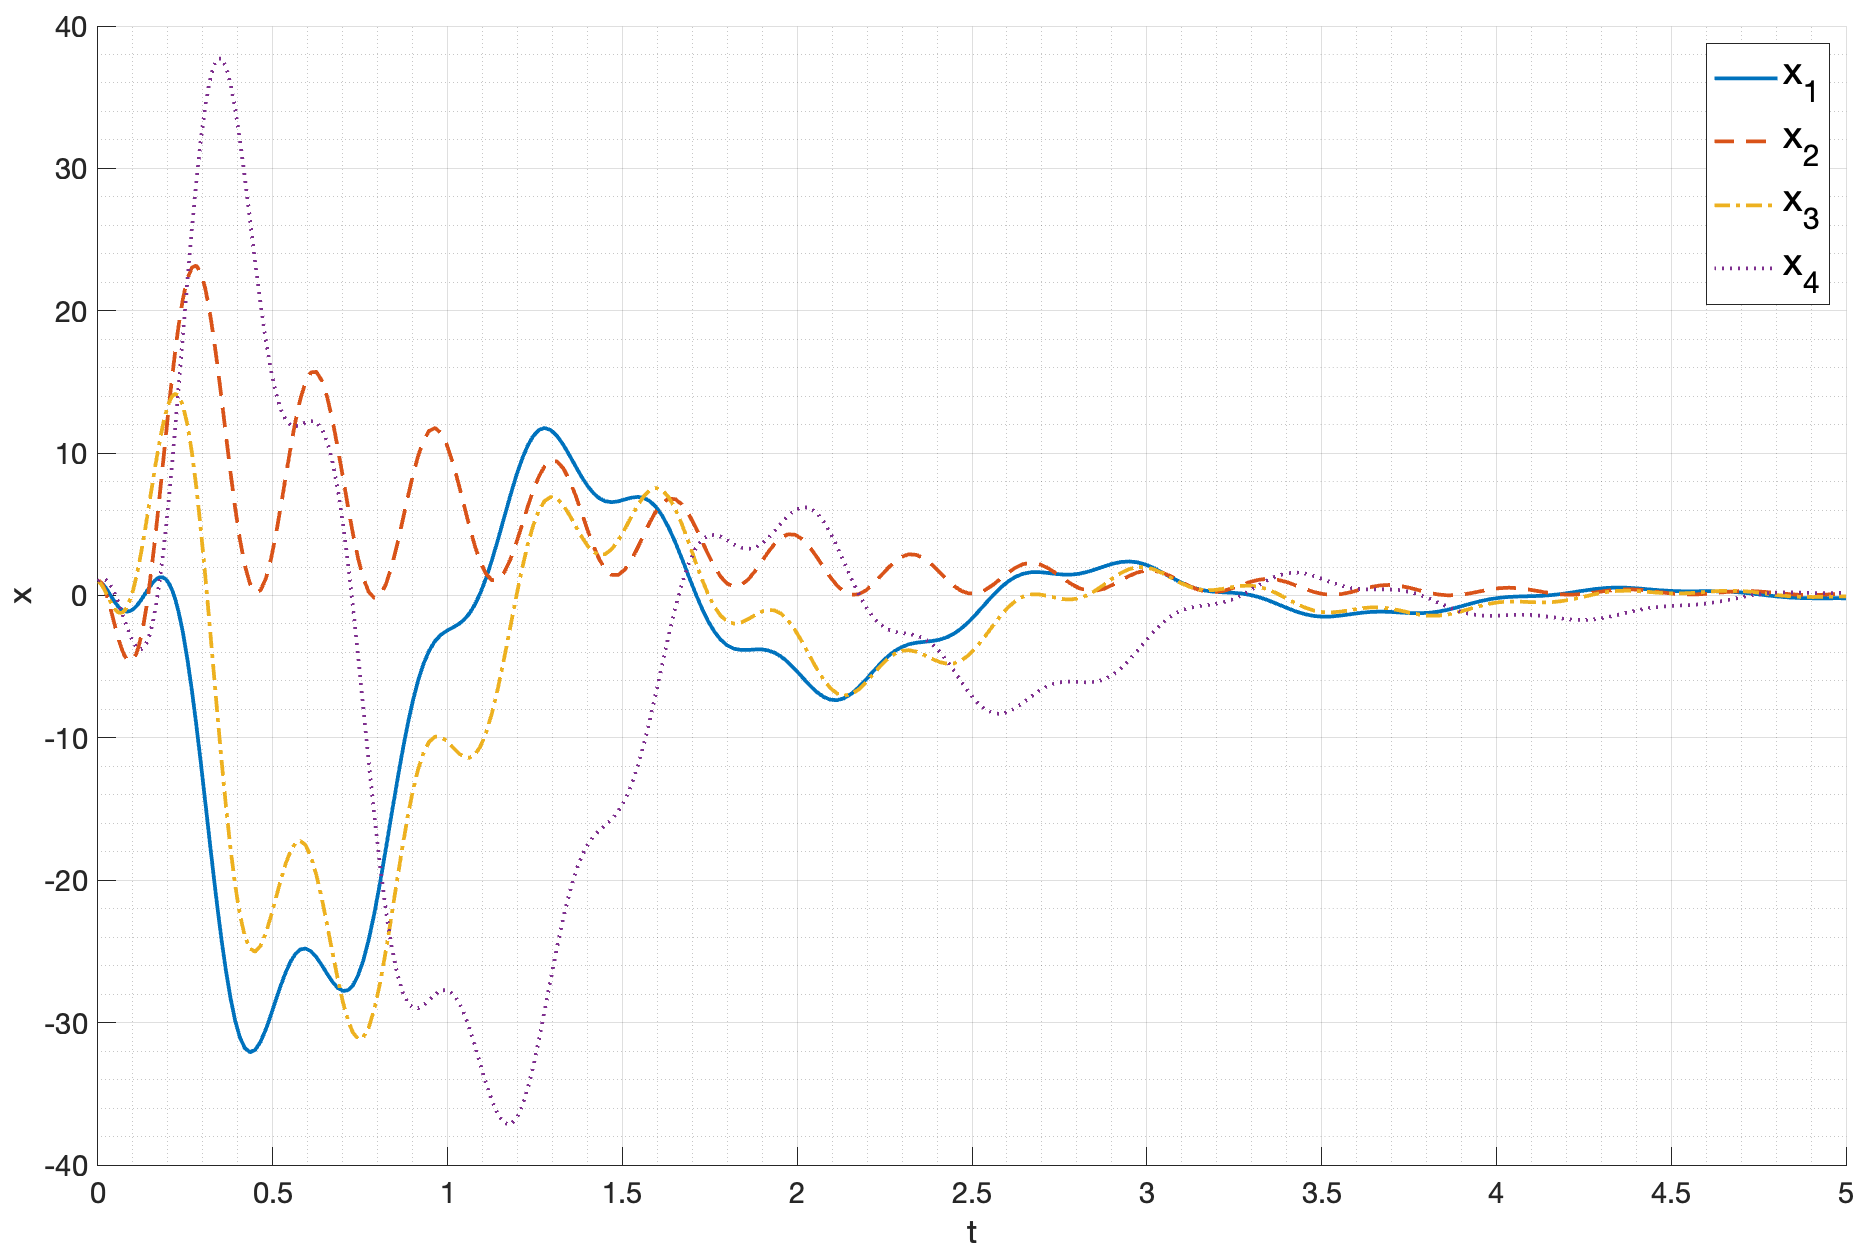
\includegraphics[width=\textwidth]{media/plots/task2_4_x.png}
    \caption{Состояние системы $K_2$ и $L_2$}
    \label{fig:task2_2_2_x}
\end{figure}
\begin{figure}[ht!]
    \centering
    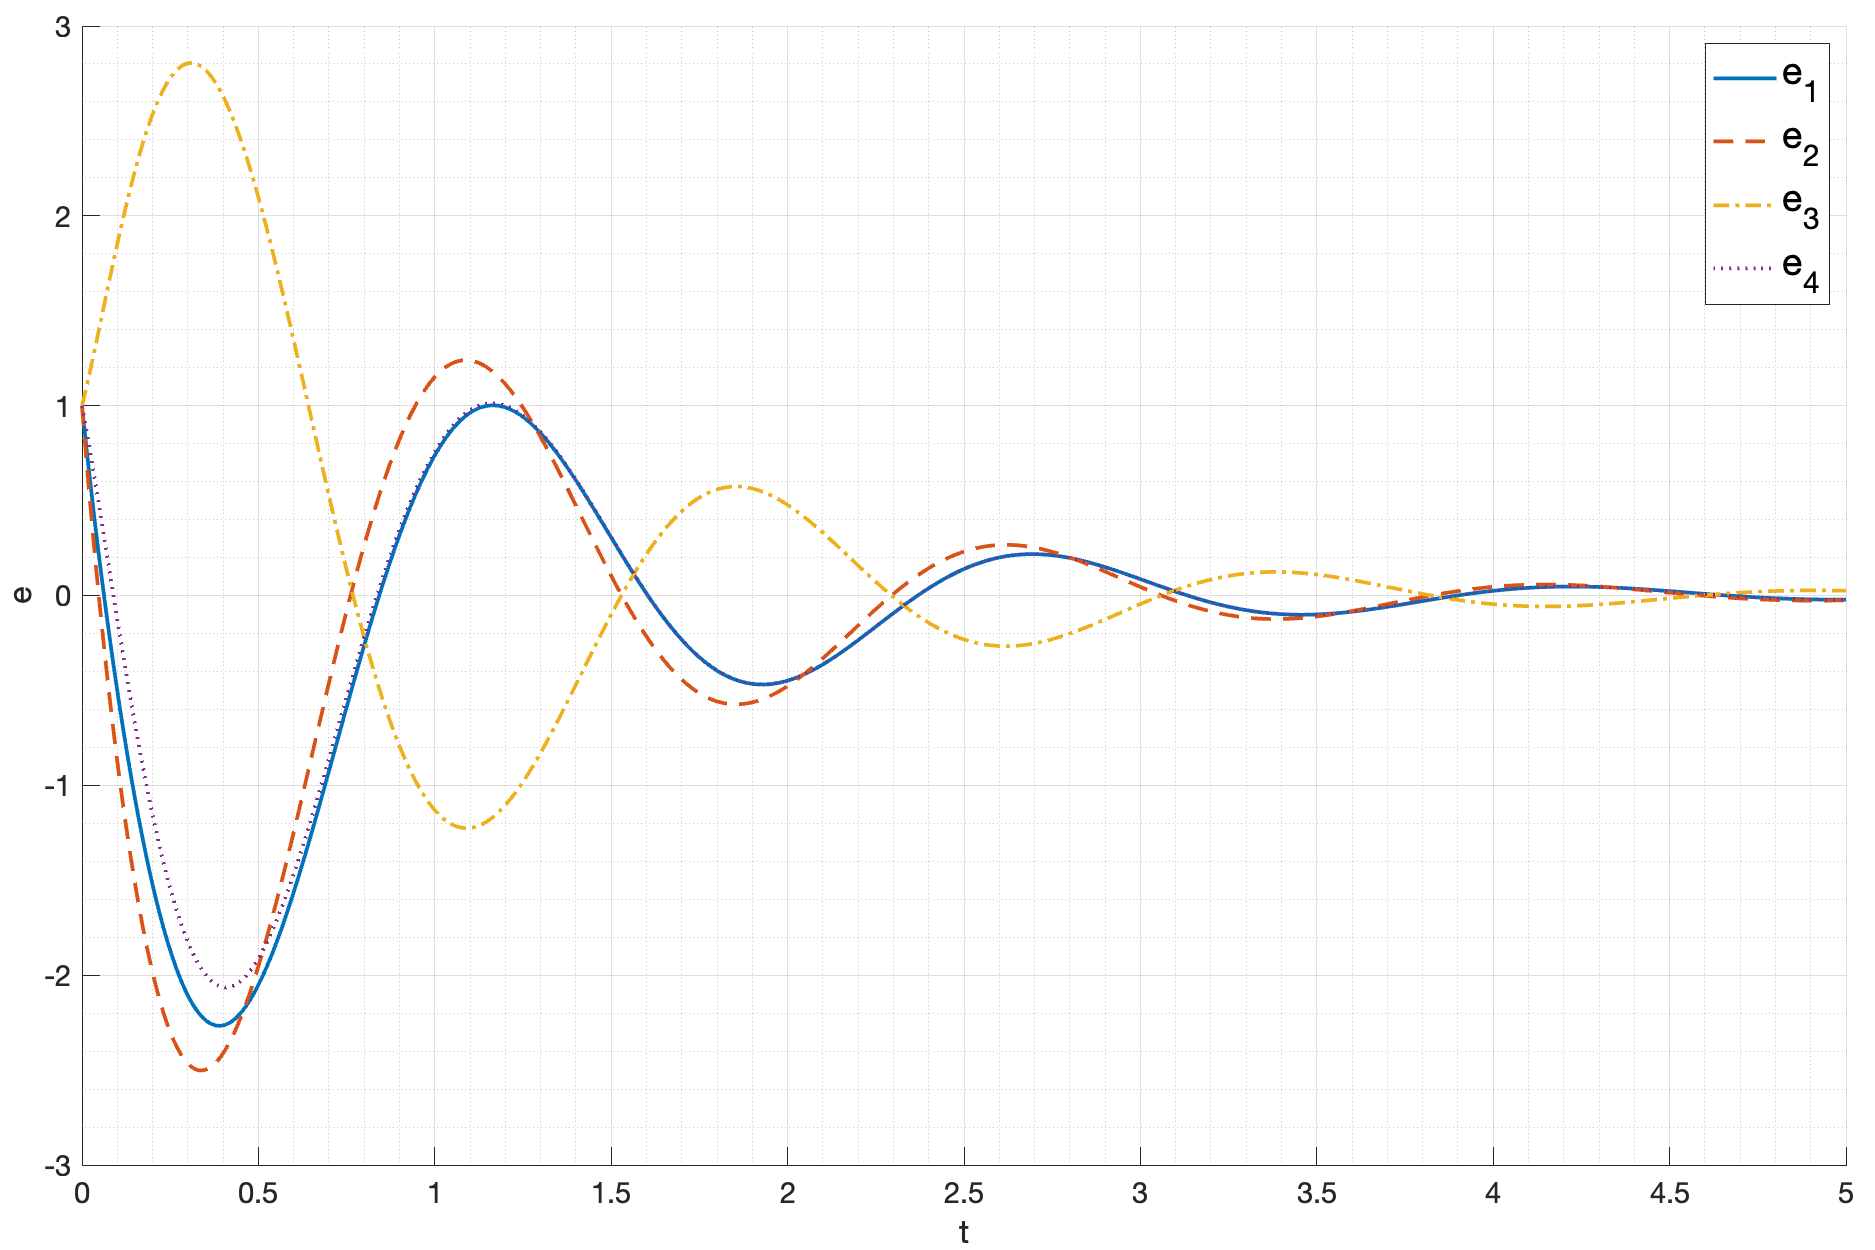
\includegraphics[width=\textwidth]{media/plots/task2_4_e.png}
    \caption{Ошибка наблюдения $K_2$ и $L_2$}
    \label{fig:task2_2_2_e}
\end{figure}
\begin{figure}[ht!]
    \centering
    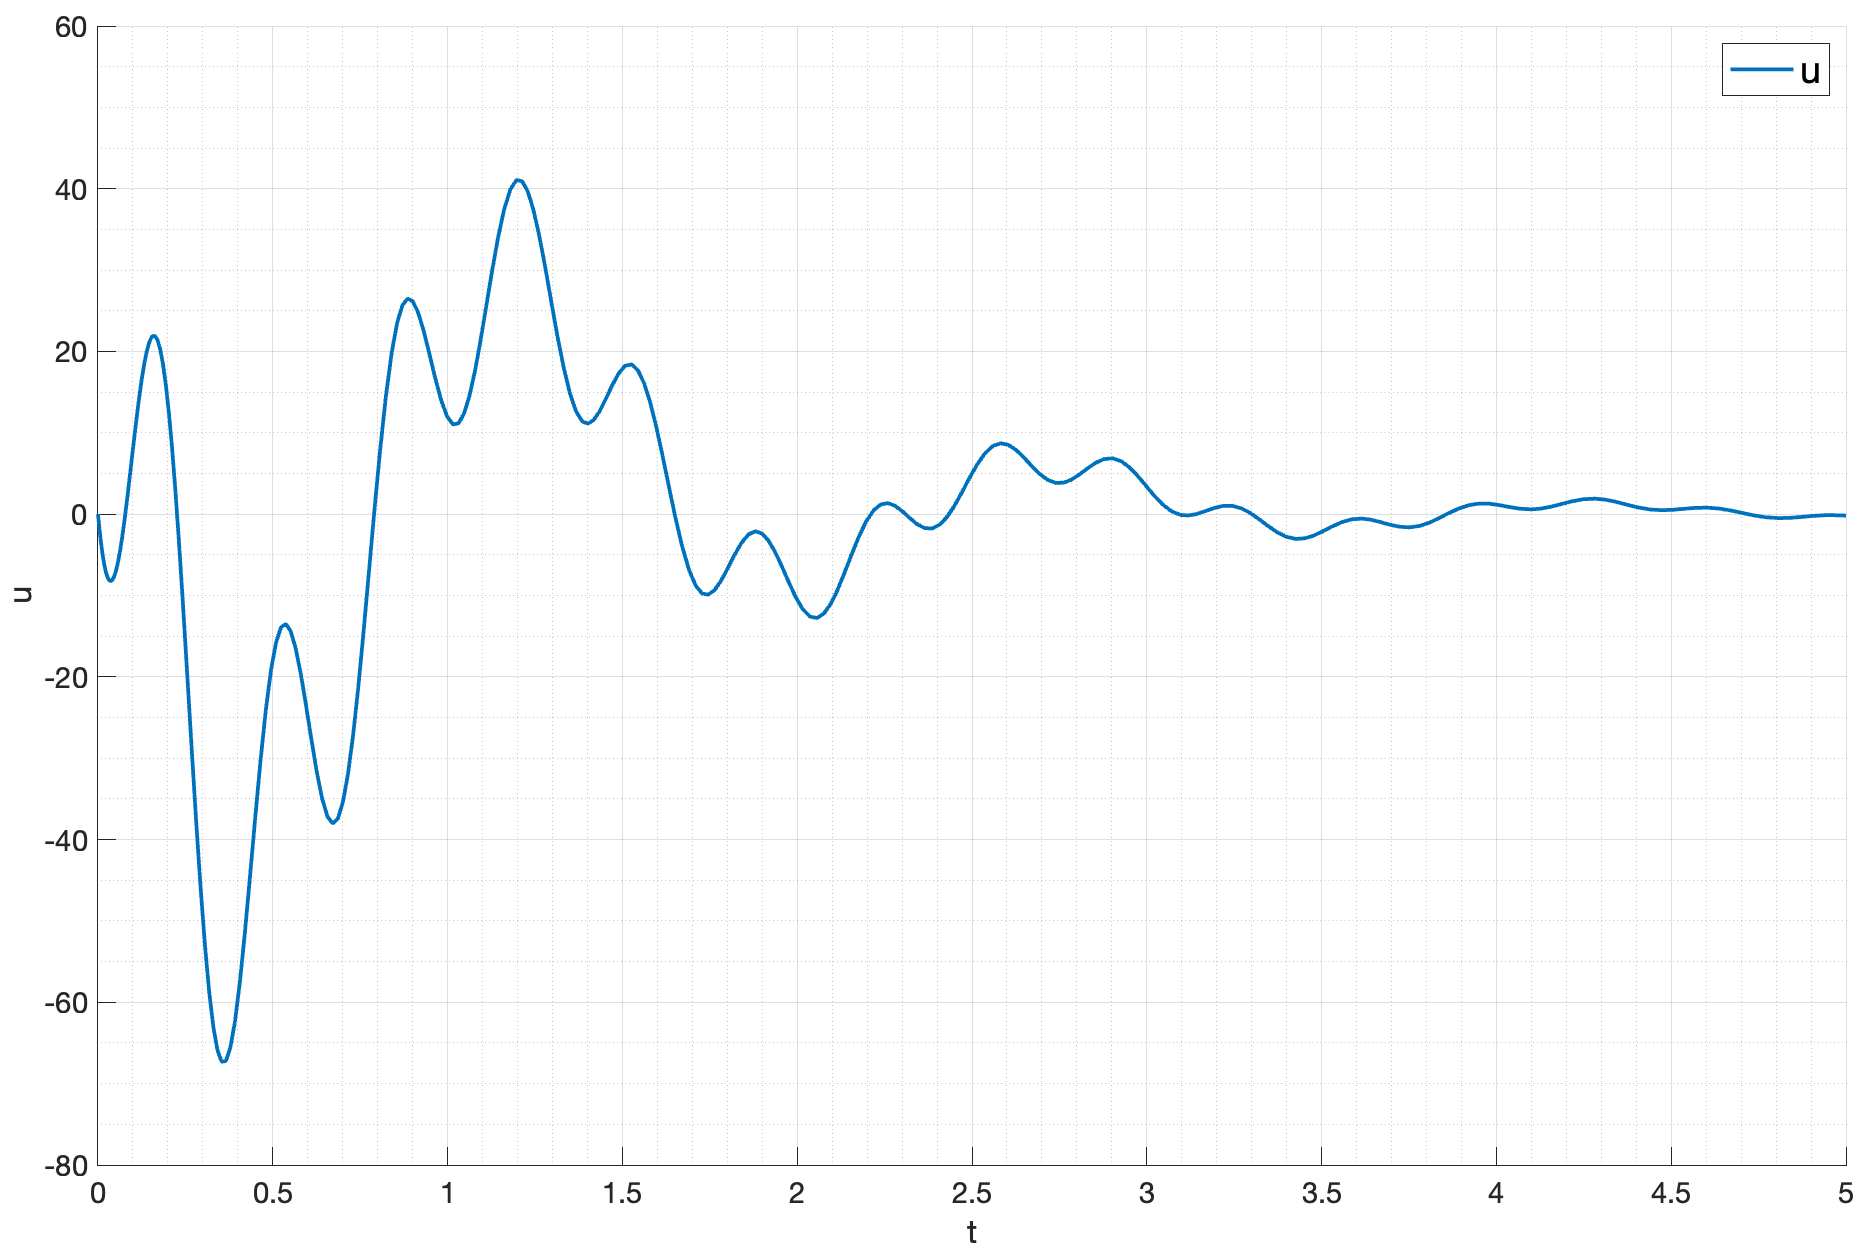
\includegraphics[width=\textwidth]{media/plots/task2_4_u.png}
    \caption{Управляющее воздействие $K_2$ и $L_2$}
    \label{fig:task2_2_2_u}
\end{figure}
\begin{figure}[ht!]
    \centering
    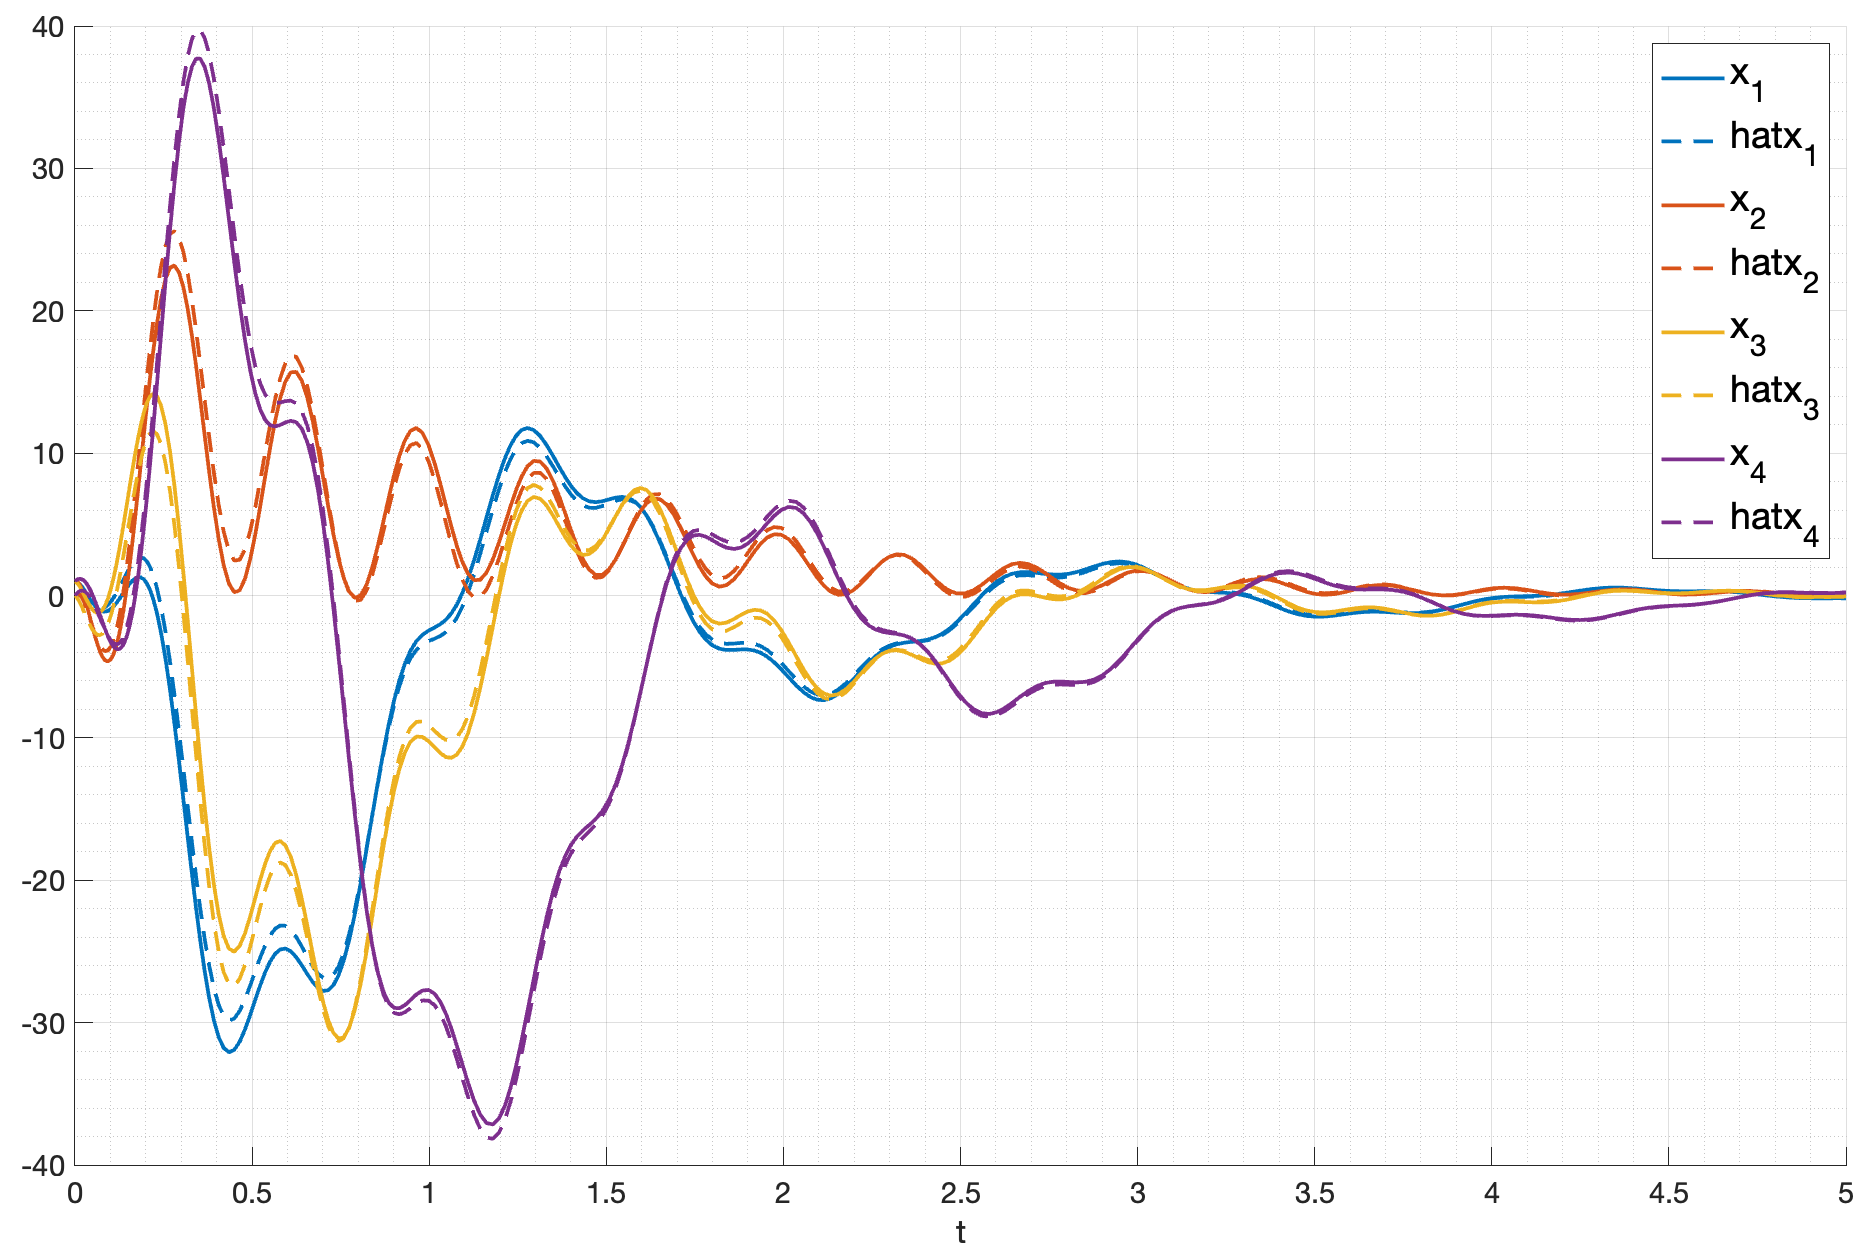
\includegraphics[width=\textwidth]{media/plots/task2_4_xh.png}
    \caption{Состояние системы и ее оценка $K_2$ и $L_2$}
    \label{fig:task2_2_2_xh}
\end{figure}
\FloatBarrier

\subsection{Выводы}
Сравнивая системы с различными регуляторами и наблюдателями, обеспечивающих разные спектры и 
степени устойчивости соответственно, можно сделать следующие выводы:
Чем больше степень устойчивости регулятора, тем быстрее состояние системы
стремится к нулю, при этом необходимо большее управляющее воздействие.
Чем больше степень устойчивости наблюдателя, тем быстрее ошибка наблюдения
стремится к нулю. 

Сравнивая системы с одинаковыми регуляторами, но разными наблюдателями, можно заметить, что
при увеличении степени устойчивости наблюдателя, состояние системы стремится к нулю быстрее. 
При \textit{слабом} наблюдении регулятор не может быстро реагировать на изменения состояния системы,
так как ошибка наблюдения стремится к нулю медленно. 

Сравнивая системы с одинаковыми наблюдателями, но разными регуляторами, можно заметить, что
при увеличении степени устойчивости регулятора, состояние системы стремится к нулю быстрее, 
чего и следовало ожидать. При этом, при \textit{сильном} наблюдении, например, как 
в случае $K_2$ и $L_1$, ошибка наблюдения сходится к нулю очень быстро, 
но состояние системы не может быстро стремиться к нулю, так как регулятор обладает 
недостаточной степенью устойчивости.    

Таким образом, можно сделать вывод, что время сходимости системы зависит от
степени устойчивости регулятора и наблюдателя, а также от их соотношения. 

P.S. \textit{Раздельные} графики состояния системы и ее оценки не приведены 
намерено, так как \textit{общие} графики достаточно наглядны, а включать в отчет еще 16 графиков 
мне не кажется целесообразным.  